%% Chapter 7 — Introduction to Serving Systems
\setcounter{chapter}{6}
\chapter{Introduction to Serving Systems}
\chaptersubtitle{Part 2 begins — online, batch, streaming, and the language of fast: tails, promises, queues, formats}

\begin{calloutbox}{tbbblue}{tbbbluefill}
{\normalsize\bfseries\color{tbbblue}Learning objectives}\par\vspace{3pt}
\begin{tbbitemize}
  \item Diagnose, from one argument in a team chat, why a service without an SLO turns every complaint into an outage and every quiet day into a coincidence — and why "the average is 182 ms" describes literally nobody.
  \item Classify a workload into \textbf{online, batch, or streaming} inference by asking "who is waiting, and for what?", and state what each mode optimizes, tolerates, and finds hard.
  \item Read and report latency as a distribution: percentiles (p50/p95/p99), why tails multiply under fan-out (the tail at scale), and how naive load-testing tools lie (coordinated omission).
  \item Write a complete SLO — SLI, target, window, load, cost ceiling — derive its error budget, and use the budget as a launch/freeze policy rather than a wish.
  \item Size a fleet with \textbf{Little's Law} (L = λ·W) and the utilization hockey stick: compute replicas from measured per-replica capacity, add headroom on purpose, and price the result honestly.
  \item Choose and convert model artifacts — pickle's code-on-load hazard vs. safetensors, eager vs. TorchScript vs. ONNX vs. compiled engines — and explain why conversion is a CI step, never a startup step.
\end{tbbitemize}
\end{calloutbox}

\vspace{3.5pt}

\begin{calloutbox}{tbbteal}{tbbtealfill}
{\normalsize\bfseries\color{tbbteal}Key terms}\par\vspace{3pt}
online / batch / streaming inference · latency percentile (p50 · p95 · p99) · the tail at scale · coordinated omission · SLI · SLO · SLA · error budget · Little's Law (L = λW) · utilization ρ · M/M/1 · the knee · headroom · servable artifact · safetensors · TorchScript / torch.export · ONNX · TensorRT engine · GGUF
\end{calloutbox}

\vspace{3.5pt}

\begin{calloutbox}{tbblightgray}{tbbboxfill}
{\normalsize\bfseries\color{tbbink}Chapter outline}\par\vspace{3pt}
\textbf{7.1} The argument, and the number nobody experienced    \textbf{7.2} Three inference modes    \textbf{7.3} Latency is a distribution — reading the tail    \textbf{7.4} SLI, SLO, SLA, and the error budget    \textbf{7.5} Queues: Little's Law and the hockey stick    \textbf{7.6} Model formats and conversion paths    \textbf{7.7} Lab: the project proposal — followed by a summary, exercises, and further reading.
\end{calloutbox}

\section{The Argument, and the Number Nobody Experienced}

Part 1 ended with something real: a model server in a container, scheduled by Kubernetes, loading weights from an object store, reachable through a load balancer, inside a locked-down network. It runs. Part 2 opens with the question that runs the next six weeks: \textbf{is it any good?} — and with the uncomfortable discovery that, as of this morning, your team does not have a number for "good." It has opinions. Here is what opinions look like in production; the transcript is a composite, but every engineering team that skipped this chapter has lived it.

\subsection*{Exhibit A: the argument}

\begin{terminalbox}
\begin{Verbatim}[breaklines=true,breakanywhere=true,fontsize=\small,formatcom=\color{tbbtermfg},codes=\tbbcodeactive]
[tue 10:12] pm     users are saying the demo "feels slow"
[tue 10:14] eng    avg latency is 182ms. that's fast. dashboard is green
[tue 10:31] pm     the CEO tried it in the all-hands. it spun for 4 seconds
[tue 10:33] eng    works fine for me?? just tried it. instant
[tue 11:02] cs     two pilot customers asked if "slow is normal for AI"
[tue 11:05] eng    define slow. compared to what? at what load?
[tue 11:06] pm     ...
[tue 11:06] eng    ...
[wed 09:00] cto    what did we actually PROMISE them?
[wed 09:04] pm     nothing. we never promised anything.
[wed 09:05] cto    then everything is a breach, and nothing is. fix that.
\end{Verbatim}
\end{terminalbox}
\figcaption{Exhibit 7-A  The argument. Every statement in it is true, which is exactly the problem: with no agreed number, every complaint is an outage and every quiet day is a coincidence.}

Do the autopsy before reading on, because the failure is subtle: \textbf{nobody in the transcript is wrong.} The engineer's 182 ms average is real. The CEO's 4 seconds is real. "Works fine for me" is real. They are all reading the same service and reporting different truths, because a service's speed is not a number — it is a \textbf{distribution} — and each person sampled a different part of it. The PM sampled complaints (the tail, self-selected); the engineer sampled the mean (a summary that, we will see, describes no one); the CEO sampled once, live, with witnesses (and one sample from a distribution with a heavy tail is a lottery ticket). The CTO's Wednesday line is the whole of Section 7.4 in one sentence: without a stated target there is no difference between fine and broken — \textit{"then everything is a breach, and nothing is."}

\subsection*{Exhibit B: the number nobody experienced}

Now watch the same service stop being a matter of opinion. One properly run load test later (§7.3 covers "properly" — it has teeth), the team has this report:

\begin{terminalbox}
\begin{Verbatim}[breaklines=true,breakanywhere=true,fontsize=\small,formatcom=\color{tbbtermfg},codes=\tbbcodeactive]
$ python report.py results.json     # 10,000 requests, tuesday 10:00-10:30
requests      10,000     errors  0.4%  (23x 504, 17x 502)
mean          182 ms     <- the dashboard number
p50            92 ms     <- half of all users: this or better
p90           220 ms
p95           340 ms
p99         2,140 ms     <- 100 users today: worse than this
p99.9       4,810 ms     <- 10 users: ~5 seconds. hi, CEO
max         9,400 ms
\end{Verbatim}
\end{terminalbox}
\figcaption{Exhibit 7-B  The same service as Exhibit 7-A, as a distribution. The mean (182 ms) sits between p50 and p90 — a summary statistic that no actual user experienced, dragged upward by a tail it fails to describe.}

Read it as a translation of the argument. \textit{"Avg is 182 ms"} — true, and useless: the mean of a right-skewed distribution is a fiction that sits where no user lives; half the users did better than 92 ms and the unlucky hundred did worse than 2.1 s. \textit{"Works fine for me"} — of course it did: at p50, most single samples do. \textit{"The CEO spun for 4 seconds"} — he drew somewhere past p99.9, which on 10,000 requests is ten real people, and at 200,000 requests a day is two hundred people, every day, forever. \textit{"Two customers asked if slow is normal"} — the tail is not an edge case; it is a \textbf{daily audience}. This is why serving systems speak in percentiles and never in averages, and why every benchmark, SLO, and dashboard for the rest of this course reports p50/p95/p99 — a discipline this chapter now builds from the ground up.

\subsection*{Speed is revenue: the classics}

\begin{calloutbox}{tbbamber}{tbbamberfill}
{\normalsize\bfseries\color{tbbamberdark}Three experiments every serving engineer can cite from memory}\par\vspace{3pt}
\begin{tbbitemize}
  \item \textbf{Amazon, 2006 (Greg Linden):} injecting +100 ms of artificial delay into page loads measurably dropped sales — the folklore figure is \textbf{−1\% of revenue per 100 ms}. The experiment that taught e-commerce to fear the millisecond.
  \item \textbf{Google, 2009 ("Speed Matters," Jake Brutlag):} slowing search results by +400 ms reduced searches per user by \textbf{−0.59\%} — and the effect \textit{persisted after the delay was removed}: slowness taught users to search less.
  \item \textbf{Google, 2006 (Marissa Mayer at Web 2.0):} users asked for 30 results per page; delivering them cost \textasciitilde{}+500 ms — and traffic dropped \textbf{\textasciitilde{}20\%}. Users prefer less, faster.
\end{tbbitemize}

Caveats stated honestly: these are 2000s-era web numbers, and your mileage will vary. But the direction has replicated for two decades, and the asymmetry is the point — users notice delay far more than they notice its absence. Latency is not an engineering vanity metric; it is a line item.
\end{calloutbox}

\vspace{3.0pt}

\subsection*{The hinge: what you own, and what you owe}

Figure 7-1 places this chapter. Below the line is Part 1 — the platform: rented compute whose true nature you can interrogate (Chapter 2), containers built from namespaces and cgroups (Chapters 3–4), a reconciling scheduler (Chapter 5), and state, doors, and perimeters (Chapter 6). All of it is now \textit{assumed}: from this week on, "deploy it" is a sentence you already know how to execute. Above the line is Part 2 — the serving system: the same deployment, now judged as a product. One request enters at the client (where the only clock that matters starts), crosses the gateway you built in Week 6, waits in a queue, gets batched, runs through a runtime executing some format of your model, and returns. Every section of this chapter is one of the labeled knobs on that path.

\begin{tbbfigure}
  \adjustbox{max width=0.94\linewidth,max totalheight=0.46\textheight}{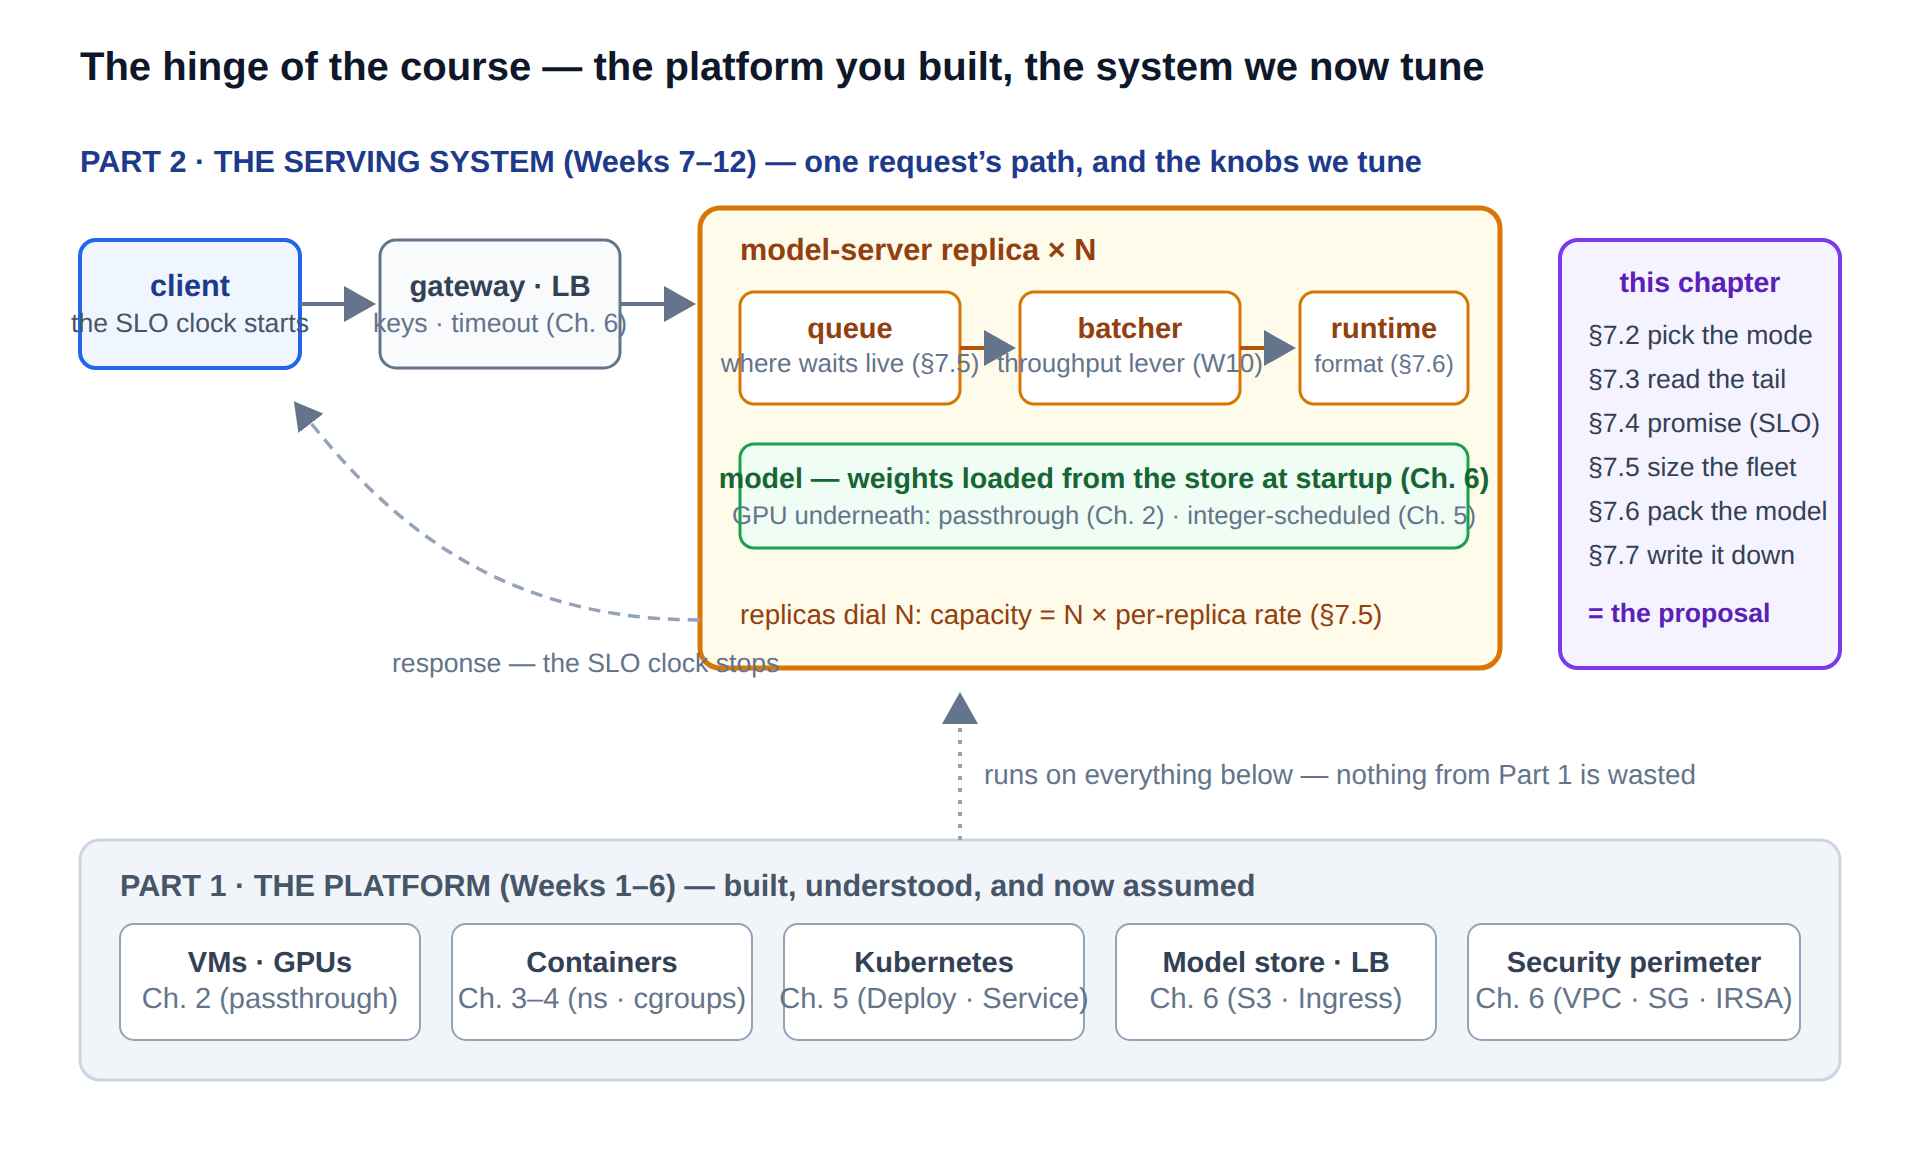
\includegraphics{figures/fig7-1_hinge.png}}\\[3pt]
  \figcaption{Figure 7-1  The hinge of the course. Part 1 built the platform below the line; Part 2 tunes the serving system above it. The chapter's sections annotate the request path: mode (§7.2), tail (§7.3), promise (§7.4), fleet (§7.5), format (§7.6), proposal (§7.7).}
\end{tbbfigure}

This is also proposal week — the team project's first deliverable is due (§7.7) — and that is not an administrative coincidence. The proposal is one page that answers, in numbers, exactly the questions Exhibit 7-A's team could not: what will you serve (§7.6's artifact), in which mode (§7.2), promising what (§7.4's SLO), at what load, on what fleet (§7.5), under what monthly ceiling (Chapter 1's cost lens)? Everything between here and §7.7 is the working material for those blanks — this chapter is, quite literally, the assignment.

\subsection*{Vocabulary for the chapter}

\begin{tbbtablewrap}
  \begin{tabular}{@{}>{\raggedright\arraybackslash}m{\dimexpr 0.2660\tbltextwidth-2\tabcolsep\relax} >{\raggedright\arraybackslash}m{\dimexpr 0.7340\tbltextwidth-2\tabcolsep\relax}@{}}
  \arrayrulecolor{tbbnavy}\specialrule{1pt}{0pt}{0pt}
  \rowcolor{tbbtablehead}{\centering \bfseries\color{tbbnavy}Term} & {\centering \bfseries\color{tbbnavy}Meaning} \\
  \arrayrulecolor{tbbnavy}\specialrule{0.7pt}{0pt}{2pt}
  {\textbf{online / batch / streaming}} & {The three inference modes, split by "who is waiting": a person per request / nobody / a person watching results flow (§7.2).} \\
  \arrayrulecolor{tbbtableborder}\hline
  {\textbf{percentile (pN)}} & {The latency such that N\% of requests were at least that fast. p99 = the experience of your unluckiest 1\% — a real crowd, daily.} \\
  \arrayrulecolor{tbbtableborder}\hline
  {\textbf{the tail at scale}} & {Dean \& Barroso's observation: under fan-out, rare slowness becomes common — 1\% slow leaves × 100-way fan-out = 63\% slow requests (§7.3).} \\
  \arrayrulecolor{tbbtableborder}\hline
  {\textbf{coordinated omission}} & {The classic load-testing bug: a closed-loop tester politely stops sending while the server stalls, then reports the stall-free percentiles (§7.3).} \\
  \arrayrulecolor{tbbtableborder}\hline
  {\textbf{SLI}} & {Service Level Indicator — the carefully defined measurement ("fraction of requests under 500 ms, at the gateway"). What is happening. (§7.4)} \\
  \arrayrulecolor{tbbtableborder}\hline
  {\textbf{SLO}} & {Service Level Objective — the target you set yourself over a window, at a stated load. What we promise ourselves. (§7.4)} \\
  \arrayrulecolor{tbbtableborder}\hline
  {\textbf{SLA}} & {Service Level Agreement — the external contract with money attached; always looser than the SLO. (§7.4)} \\
  \arrayrulecolor{tbbtableborder}\hline
  {\textbf{error budget}} & {1 − SLO target, as spendable unreliability: 99.9\% over 30 days = \textasciitilde{}43 minutes. A launch/freeze policy, not a report card (§7.4).} \\
  \arrayrulecolor{tbbtableborder}\hline
  {\textbf{λ, W, L}} & {Arrival rate (req/s), time in system (s), and number in flight — joined by Little's Law, L = λ·W, for any stable system (§7.5).} \\
  \arrayrulecolor{tbbtableborder}\hline
  {\textbf{utilization ρ · headroom}} & {Offered load ÷ capacity. Latency explodes as ρ → 1 (the hockey stick), so online fleets buy headroom on purpose (§7.5).} \\
  \arrayrulecolor{tbbtableborder}\hline
  {\textbf{servable artifact}} & {What actually ships: weights (safetensors) + config + tokenizer, versioned in the model store (Ch. 6), in a format the runtime executes (§7.6).} \\
  \arrayrulecolor{tbbnavy}\specialrule{1pt}{2pt}{0pt}
  \end{tabular}\par
  \figcaption{Table 7-1  Working vocabulary for this chapter}
\end{tbbtablewrap}

\begin{calloutbox}{tbbpurple}{tbbpurplefill}
{\normalsize\bfseries\color{tbbpurple}Think About It}\par\vspace{3pt}
\begin{tbbitemize}
  \item Replay Exhibit 7-A at your favorite real service's scale. If p99.9 = 5 s and they serve 50 million requests a day, how many five-second experiences happen daily? Is "p99.9" still a corner case?
  \item The engineer's dashboard was green because it charted the mean. Sketch the two or three lines the dashboard should have charted instead — and where the alert thresholds would come from. (You are designing §7.4 from scratch; check yourself after reading it.)
  \item Exhibit 7-B's error line reads "0.4\% (23× 504, 17× 502)." Using Chapter 6's status-code field guide: which of these two codes is the load balancer confessing about itself, and which is it blaming on your server — and why does the SLO in §7.4 have to count both?
\end{tbbitemize}
\end{calloutbox}

\section{Three Inference Modes: Who Is Waiting, and for What?}

The first blank in your proposal is the cheapest to fill and the most expensive to get wrong. Before any talk of frameworks or GPUs, a serving system is shaped by one question: \textbf{who is waiting on this inference, and for what?} The three answers — a person is waiting for \textit{this} answer (online); nobody is waiting (batch); a person is watching answers \textit{flow} (streaming) — produce three systems so different that they barely share an operations manual, even when the model weights are byte-identical (Figure 7-2).

\begin{tbbfigure}
  \adjustbox{max width=0.94\linewidth,max totalheight=0.46\textheight}{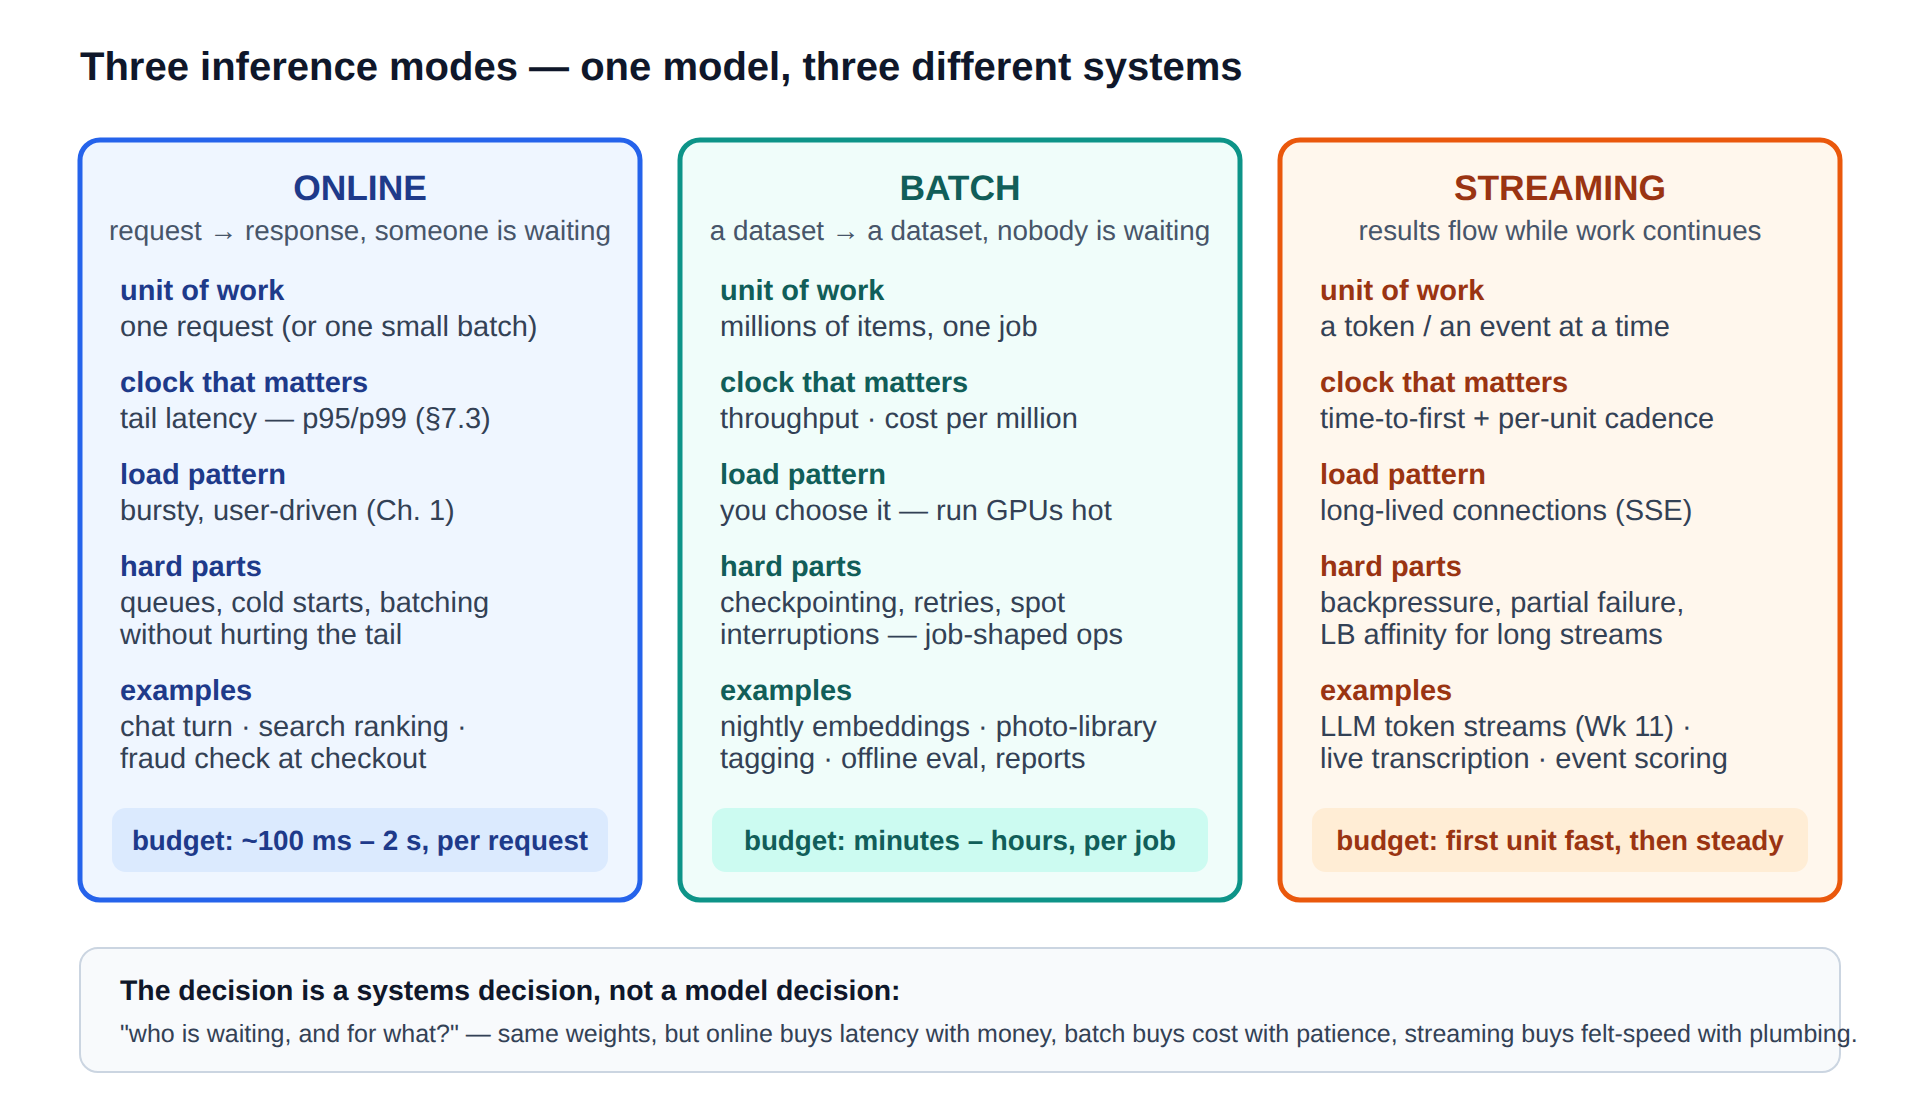
\includegraphics{figures/fig7-2_modes.png}}\\[3pt]
  \figcaption{Figure 7-2  Three inference modes. Same model, three systems: online manages tails, batch manages cost, streaming manages the feeling of speed.}
\end{tbbfigure}

\subsection*{Online: the default everyone assumes — and the mode this course is hardest on}

\textbf{Online inference} answers a live request while a human (or a paying upstream service) waits: a chat turn, a search ranking, a fraud check inside a checkout flow. Its defining physics: the unit of work is one request; the clock that matters is the \textbf{tail} of the latency distribution, because the tail is where users actually churn (§7.3); load arrives when users feel like it (bursty — Chapter 1); and capacity must therefore be provisioned \textit{ahead} of demand, which is why everything from Exhibit 1-A's queue collapse to Week 12's autoscaling lives in this mode. When this book says "serving" without qualification, it means online — the mode where every hard topic of Part 2 (batching against the tail, cold starts, SLOs, fleet sizing) earns its keep.

\subsection*{Batch: the easy mode — always check it first}

\textbf{Batch inference} runs a model over a dataset with nobody waiting: tonight, tag every photo uploaded today; every Sunday, re-embed the document corpus; before the meeting, score last quarter's claims. It is Chapter 1's "training-shaped serving," and its arrival pays a debt: Chapter 1's think box asked \textit{what gets simpler} — here is the honest, slightly embarrassing list. The tail SLO \textbf{disappears} (no one experiences p99 of a nightly job; only the deadline matters). Autoscaling \textbf{disappears} (you choose the load; there are no surprises to chase). The hockey stick of §7.5 becomes your friend instead of your enemy: with nobody waiting, you run GPUs at 95\%+ utilization on purpose — the exact opposite of the online rulebook. Failures cost retries, not users, so \textbf{spot instances} (Week 12) — interruptible capacity at a deep discount — fit batch perfectly. What remains is job-shaped engineering: checkpointing progress, idempotent retries, and one metric, \textbf{cost per million items}.

The practical rule this buys you: \textbf{the cheapest latency optimization in existence is discovering that nobody was actually waiting.} A surprising share of "we need real-time inference" requirements dissolve under the question "what happens if this answer arrives an hour later?" — and every workload you move from online to batch converts SLO engineering into a cron job. Your proposal should say explicitly which of your traffic is truly online, and route the rest to the easy mode.

\subsection*{Streaming: buying the feeling of speed with plumbing}

\textbf{Streaming inference} delivers results while the work continues — most famously the LLM token stream (the reason chat interfaces feel alive), but also live transcription and event scoring. Its clocks split in two: \textbf{time to first unit} (how long before something appears — the new "latency") and \textbf{cadence} (units per second thereafter). The trick is psychological as much as technical: an answer whose final token lands at 8 seconds \textit{feels} fast if the first token landed at 300 ms, which is why Week 11 treats time-to-first-token as a first-class SLI. The price is plumbing: long-lived connections (SSE or WebSockets) that must pass through every proxy and load balancer of Chapter 6 without buffering, \textbf{backpressure} when the consumer is slower than the producer, and partial-failure semantics (what does "retry" mean when half an answer already streamed?). We only name the mode here; its serving engine internals are Week 11's subject.

\begin{tbbtablewrap}
  \begin{tabular}{@{}>{\raggedright\arraybackslash}m{\dimexpr 0.2606\tbltextwidth-2\tabcolsep\relax} >{\raggedright\arraybackslash}m{\dimexpr 0.2447\tbltextwidth-2\tabcolsep\relax} >{\raggedright\arraybackslash}m{\dimexpr 0.2394\tbltextwidth-2\tabcolsep\relax} >{\raggedright\arraybackslash}m{\dimexpr 0.2553\tbltextwidth-2\tabcolsep\relax}@{}}
  \arrayrulecolor{tbbnavy}\specialrule{1pt}{0pt}{0pt}
  \rowcolor{tbbtablehead}{\centering \bfseries\color{tbbnavy}Ask} & {\centering \bfseries\color{tbbnavy}Online} & {\centering \bfseries\color{tbbnavy}Batch} & {\centering \bfseries\color{tbbnavy}Streaming} \\
  \arrayrulecolor{tbbnavy}\specialrule{0.7pt}{0pt}{2pt}
  {\textbf{Who waits?}} & {a person / a live upstream, per request} & {nobody — a deadline, at most} & {a person, watching results flow} \\
  \arrayrulecolor{tbbtableborder}\hline
  {\textbf{The clock}} & {tail latency (p95/p99)} & {job completion · cost per million} & {time-to-first + cadence} \\
  \arrayrulecolor{tbbtableborder}\hline
  {\textbf{Load pattern}} & {users decide (bursty)} & {you decide (schedule it)} & {long-lived, session-shaped} \\
  \arrayrulecolor{tbbtableborder}\hline
  {\textbf{Utilization stance}} & {headroom on purpose (§7.5)} & {run hot on purpose (ρ→0.95)} & {headroom + connection budgets} \\
  \arrayrulecolor{tbbtableborder}\hline
  {\textbf{A failure costs}} & {a user, immediately} & {a retry, invisibly} & {a broken stream mid-sentence} \\
  \arrayrulecolor{tbbnavy}\specialrule{1pt}{2pt}{0pt}
  \end{tabular}\par
  \figcaption{Table 7-2  Choosing the mode — five questions that decide it}
\end{tbbtablewrap}

One last honesty: real products are \textbf{mixtures}. A chat product streams its answers (streaming), pre-computes embeddings for retrieval nightly (batch), and ranks candidate documents inside the request path (online). The proposal template therefore asks for your traffic \textit{decomposition}, not a single checkbox — and the decomposition is where reviewers first see whether a team has actually thought about its system.

\begin{calloutbox}{tbbpurple}{tbbpurplefill}
{\normalsize\bfseries\color{tbbpurple}Think About It}\par\vspace{3pt}
\begin{tbbitemize}
  \item A team says: "our recommendation model must be online — the homepage needs it." Their homepage renders for each user at most once per session, from a profile that changes daily. Argue the batch redesign: what is precomputed, what tiny online component (if any) remains, and what happened to the SLO?
  \item For an LLM chat product, write down the two streaming clocks (time-to-first-token, tokens/second) that would make chat feel instant vs. broken to you personally. Now check your intuition against any chat service you use — can you estimate its numbers with a stopwatch?
  \item Which mode is a nightly job that MUST finish by 6 a.m.? It has no per-item latency target, but it has a deadline — so is "nobody is waiting" quite true? What is the SLO-shaped sentence for this job? (§7.4 will give you the vocabulary to write it.)
\end{tbbitemize}
\end{calloutbox}

\section{Latency Is a Distribution — Reading the Tail}

Exhibit 7-B already made the argument by ambush; this section makes it a discipline. A latency number without a percentile attached is not information — it is Exhibit 7-A waiting to happen. Figure 7-3 is the mental picture to keep: every service's latency is a \textbf{right-skewed distribution} with a long tail, and the three families of facts below — how to read it, how it multiplies, and how tools lie about it — are the working knowledge of everyone who runs serving systems for a living.

\begin{tbbfigure}
  \adjustbox{max width=0.94\linewidth,max totalheight=0.46\textheight}{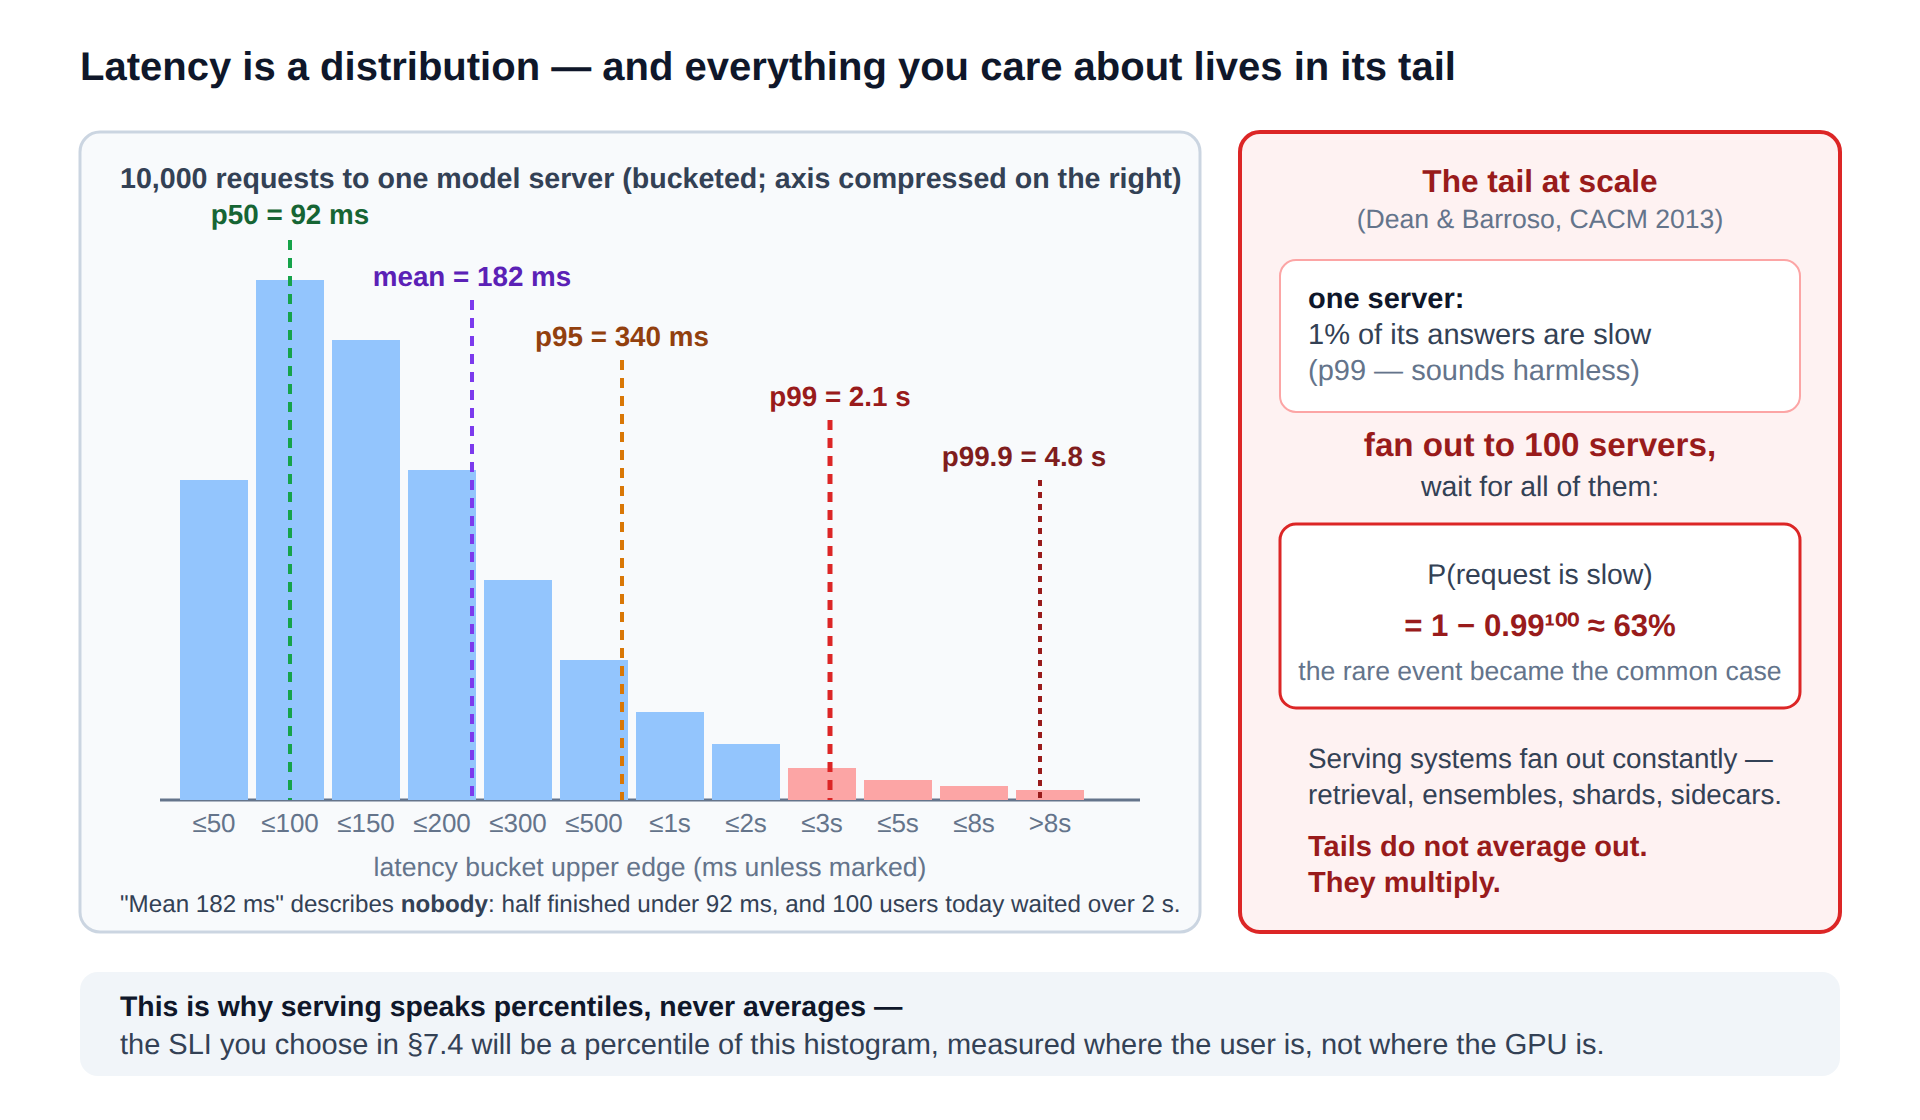
\includegraphics{figures/fig7-3_tail.png}}\\[3pt]
  \figcaption{Figure 7-3  The latency distribution behind Exhibit 7-B, with its percentile markers — and, right, the tail-at-scale arithmetic that makes rare slowness a common experience under fan-out.}
\end{tbbfigure}

\subsection*{The grammar of percentiles}

\textbf{pN is the latency that N\% of requests beat.} p50 (the median) is the typical experience; p95 and p99 are the unlucky 5\% and 1\%; p99.9 is the crowd your CEO samples during all-hands demos. Four grammar rules keep you honest. First, \textbf{the mean is not a percentile} and for skewed distributions describes nobody — it is pulled up by the tail while telling you nothing about the tail's size; Exhibit 7-B's mean of 182 ms sat between p50 and p90, experienced by no one. Second, \textbf{percentiles are properties of a window and a population}: "p99 = 2.1 s" means nothing without \textit{measured where, over what period, at what load} — tuesday-morning p99 and black-friday p99 are different facts. Third, \textbf{percentiles do not add}: if step A has p99 = 100 ms and step B has p99 = 100 ms, the pipeline's p99 is \textit{not} 200 ms — the unlucky 1\% of A and of B are mostly different requests (the pipeline's p99 is somewhere between, and only the full distributions can say where). Fourth — the operational corollary — \textbf{you cannot average percentiles}: the mean of ten replicas' p99s is not the fleet's p99. To aggregate across replicas or time you must merge \textit{histograms}, which is exactly why serious metrics systems (Week 14's Prometheus) ship latency as histogram buckets rather than pre-chewed percentiles.

\subsection*{The tail at scale: rare slowness, multiplied}

Why do practitioners obsess over p99 rather than p50? Beyond "the tail is where users churn," there is a structural amplifier, named in the paper every serving engineer eventually reads — Dean and Barroso's \textbf{"The Tail at Scale"} (CACM, 2013). Modern serving fans out: one user request touches a retrieval shard here, an embedding service there, a ranker, a safety filter, a template renderer. Suppose each downstream call is slow only 1\% of the time (p99 misbehaving). Fan out to 100 such calls and wait for all of them: the probability the user's request hits at least one slow call is 1 − 0.99¹⁰⁰ ≈ \textbf{63\%}. Each component's \textit{rare} event has become the user's \textit{common} experience — tails do not average out; they multiply. This single computation explains an entire genre of serving architecture: keeping fan-out shallow, setting per-call timeouts tighter than the user deadline (Chapter 6's gateway discipline), and the paper's famous mitigation, \textbf{hedged requests} — send the same query to a second replica after a delay and take the first answer, converting the tail of one server into the \textit{minimum} of two. (Hedging trades duplicate work for tail latency: the serving triangle again, spending cost to buy the tail.)

\subsection*{How load tests lie: coordinated omission}

Your percentiles are only as honest as the tool that measured them, and the most common measurement bug in the industry has a name worth knowing: \textbf{coordinated omission} (coined by Gil Tene, whose HdrHistogram and wrk2 exist to fix it). The bug: a \textit{closed-loop} load tester keeps a fixed number of requests in flight — each virtual user sends, waits for the response, then sends again. When the server stalls, the tester's virtual users are all stuck waiting — so the tester \textit{politely stops generating load exactly when the server is at its worst}, then reports percentiles computed only over the requests it happened to send. The stall barely appears in the data. Real users are not so polite: they keep arriving during the stall, and their true waiting time includes it. Transcript 7-1 shows the difference on a deliberately rigged server:

\begin{terminalbox}
\begin{Verbatim}[breaklines=true,breakanywhere=true,fontsize=\small,formatcom=\color{tbbtermfg},codes=\tbbcodeactive]
# the server is rigged to stall 1.5 s every 60 s (a "GC pause")
$ wrk -t4 -c64 -d120s http://svc/predict      # closed loop, 64 in flight
  Latency   p50 11ms    p99 13ms    max 1.51s
# during each stall only the 64 in-flight requests wait; 64 samples out
# of ~60,000/window = 0.1% -> the p99 never sees the stall. "all green."
$ wrk2 -t4 -c64 -R1000 -d120s http://svc/predict   # open loop: 1,000/s,
  Latency   p50 12ms    p99 1,140ms p99.9 1.49s    # arrivals never pause
# 1,500 requests' worth of demand arrived DURING each stall and queued.
# wrk2 charges the server for the wait, as a user's clock would.
\end{Verbatim}
\end{terminalbox}
\figcaption{Transcript 7-1  Coordinated omission, demonstrated. Same server, same stall: the closed-loop tool reports p99 = 13 ms; the open-loop tool reports p99 = 1.14 s. Only one of them describes your users.}

The moral is not "wrk bad, wrk2 good" — it is that \textbf{a load generator models an arrival process}, and you must choose the model that matches reality. Closed-loop (fixed concurrency) answers "what can this server sustain when clients wait their turn?" — a fine question for capacity probing. Open-loop (fixed arrival rate, like wrk2's -R or Locust's constant-throughput shape) answers "what will users experience at λ requests per second?" — the SLO question, because real arrivals do not pause out of courtesy. Week 9's lab, where you load-test your own framework-served model with Locust, will require the open-loop answer — and your Week 15 demo is graded on it.

\begin{calloutbox}{tbbpurple}{tbbpurplefill}
{\normalsize\bfseries\color{tbbx5B21B6}Box 7-1  Load-test hygiene — the checklist your numbers must survive}\par\vspace{3pt}
\begin{tbbitemize}
  \item \textbf{Warm up first, report separately.} The first requests pay one-time costs (model load, CUDA context, JIT, caches — your Chapter 2 lab measured this). Steady-state percentiles begin after warm-up; the warm-up itself is your cold-start datum (Week 12).
  \item \textbf{Open loop for SLO questions} — fixed arrival rate at (and above) target λ; closed loop only for capacity probing, labeled as such.
  \item \textbf{Long enough to fill the tail:} at 100 req/s, p99.9 is one request per 10 seconds — a 30 s test has \textasciitilde{}3 samples of it. Minutes, not seconds.
  \item \textbf{Report errors WITH latency, never separately.} A server that times out 5\% of requests has a wonderful p99 among the survivors — Exhibit 7-B prints error rate on the same card for exactly this reason. (Timeouts are the tail wearing a trench coat.)
  \item \textbf{Measure where the user is:} client-side (through the Chapter 6 gateway), not inside the pod. The queue you are most likely to miss is the one in front of your own server.
  \item \textbf{Repeat at least once.} A percentile that moves 3× between runs is telling you about your test, not your server.
\end{tbbitemize}
\end{calloutbox}

\vspace{3.0pt}

\begin{calloutbox}{tbbpurple}{tbbpurplefill}
{\normalsize\bfseries\color{tbbpurple}Think About It}\par\vspace{3pt}
\begin{tbbitemize}
  \item Your pipeline is gateway → retrieval → model → postprocess, each with p99 = 100 ms. A teammate budgets "p99 ≈ 400 ms total." Explain the two distinct errors in that sentence (one about adding percentiles, one about what dominates a pipeline's tail), and describe what data you would need to budget honestly.
  \item Compute the tail-at-scale figure for your own project's likely fan-out (retrieval + model + safety filter = 3 calls): with each at 1\% slow, what fraction of user requests hit a slow call? At what fan-out does it cross 10\%?
  \item Design a 60-second demo of coordinated omission using only sleep() in a toy server and two runs of a load tool — which numbers do you predict each run reports? (Then actually run it; it is one of this chapter's lab options.)
\end{tbbitemize}
\end{calloutbox}

\section{SLI, SLO, SLA — and the Error Budget}

The CTO's Wednesday-morning order — \textit{"what did we promise them? fix that"} — has a standard, battle-tested fix, and this course adopts it wholesale from the discipline that invented it (Google's Site Reliability Engineering; Chapter 4 of the SRE book is this week's required reading). The fix is a small ladder of three words that are constantly confused and must not be: \textbf{SLI, SLO, SLA} (Figure 7-4). Learn the ladder once and Exhibit 7-A becomes structurally impossible: every participant in that argument was missing a different rung.

\begin{tbbfigure}
  \adjustbox{max width=0.94\linewidth,max totalheight=0.46\textheight}{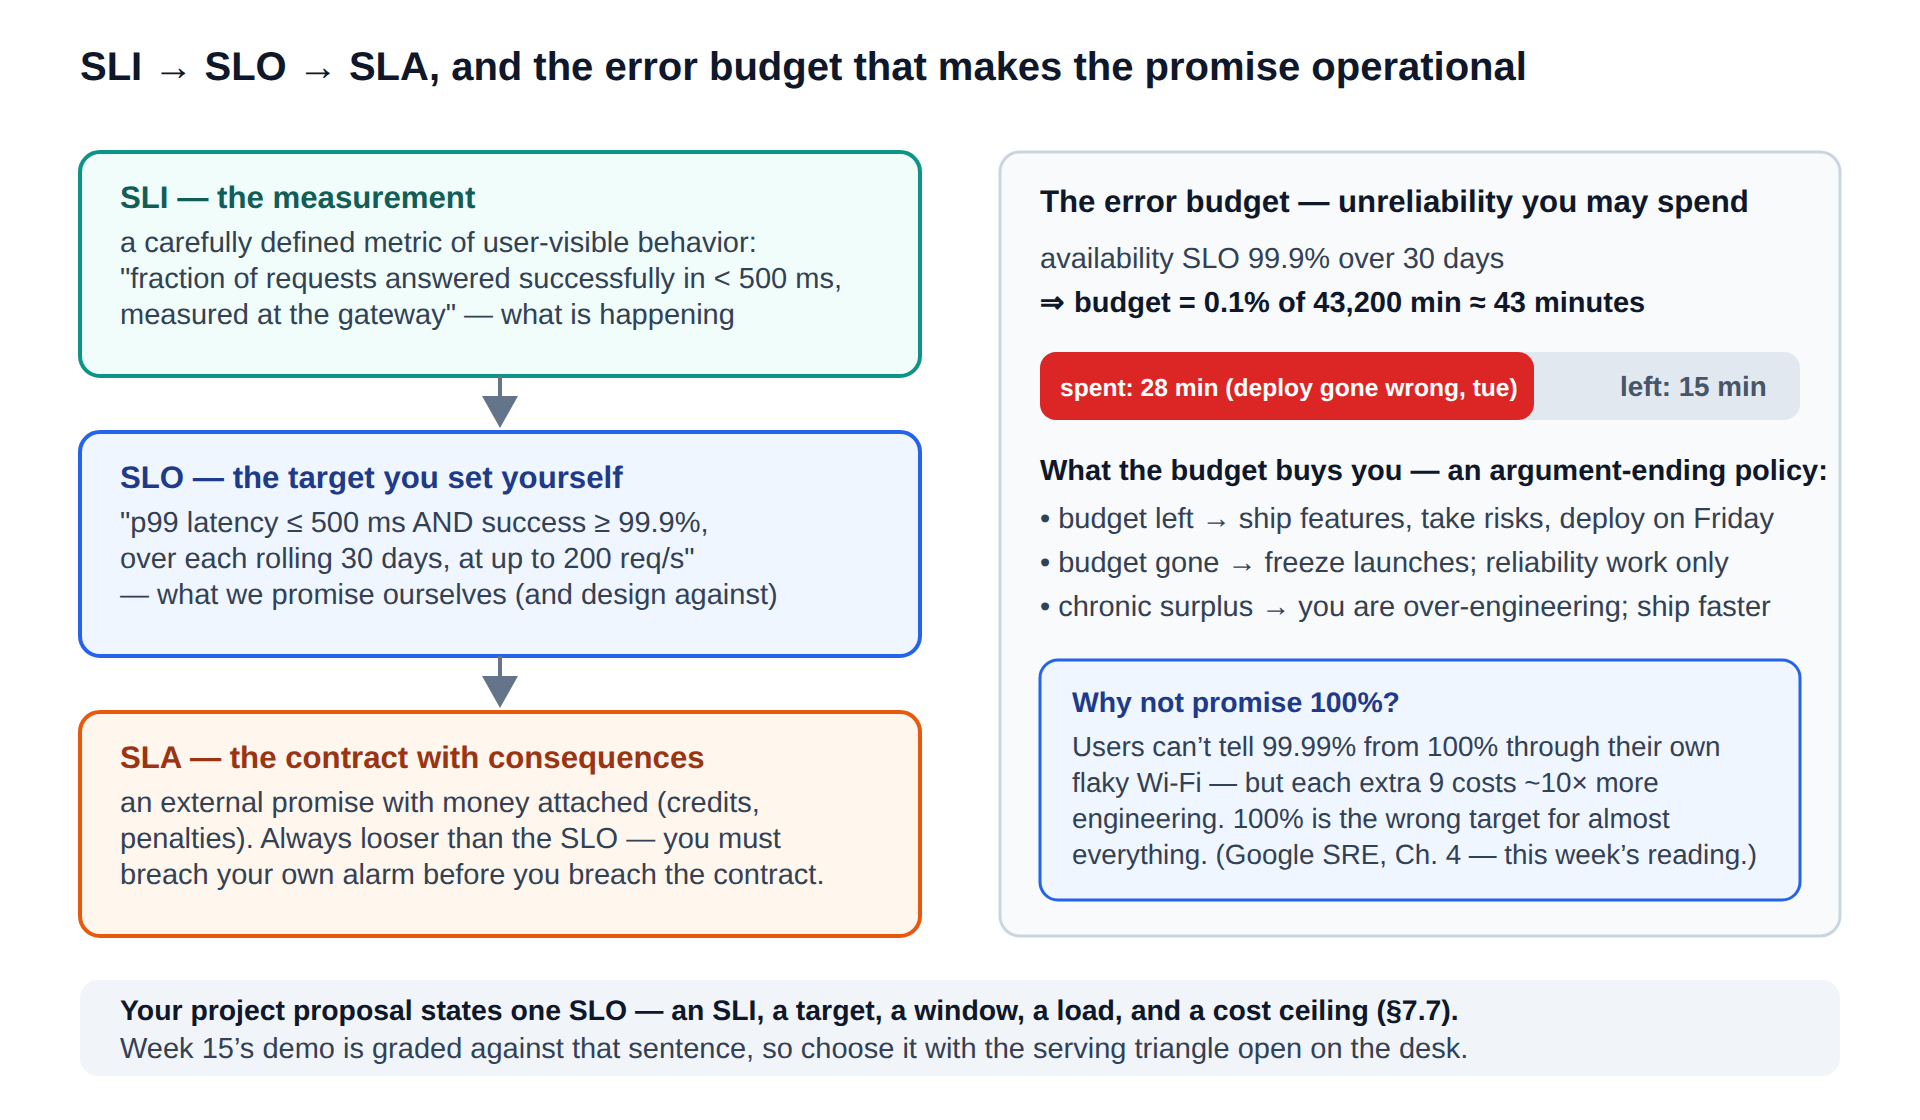
\includegraphics{figures/fig7-4_slo.png}}\\[3pt]
  \figcaption{Figure 7-4  The ladder and the budget. An SLI measures, an SLO targets, an SLA contracts — and the error budget turns the target into a policy machine.}
\end{tbbfigure}

\subsection*{SLI: measure like a user, count like an accountant}

A \textbf{Service Level Indicator} is a carefully specified measurement of user-visible behavior. The craft is in the specification: a good SLI is (a) \textbf{user-proximate} — measured where the user is, at the gateway or beyond, never inside the pod (the queue in front of your server is invisible from inside it — §7.3's hygiene rule); (b) \textbf{a ratio of good events to total events}, because ratios compose over windows and survive traffic changes ("fraction of requests answered successfully within 500 ms" rather than "average latency"); and (c) \textbf{countable without argument} — two engineers reading the definition must produce the same number. Exhibit 7-A's dashboard failed all three at once: it charted a mean (not a ratio), computed server-side (not user-proximate), of successes only (arguable). Table 7-3 is the working menu for inference services.

\begin{tbbtablewrap}
  \begin{tabular}{@{}>{\raggedright\arraybackslash}m{\dimexpr 0.2287\tbltextwidth-2\tabcolsep\relax} >{\raggedright\arraybackslash}m{\dimexpr 0.4362\tbltextwidth-2\tabcolsep\relax} >{\raggedright\arraybackslash}m{\dimexpr 0.3351\tbltextwidth-2\tabcolsep\relax}@{}}
  \arrayrulecolor{tbbnavy}\specialrule{1pt}{0pt}{0pt}
  \rowcolor{tbbtablehead}{\centering \bfseries\color{tbbnavy}SLI family} & {\centering \bfseries\color{tbbnavy}A well-formed example} & {\centering \bfseries\color{tbbnavy}The trap it avoids} \\
  \arrayrulecolor{tbbnavy}\specialrule{0.7pt}{0pt}{2pt}
  {\textbf{Availability}} & {fraction of requests answered with non-5xx, at the gateway, incl. LB-generated 502/504} & {counting only errors your code returned — the LB's 504s are user-visible failures too (Ch. 6)} \\
  \arrayrulecolor{tbbtableborder}\hline
  {\textbf{Latency}} & {fraction of successful requests completing < 500 ms at the gateway (equivalently: p99 ≤ 500 ms)} & {averaging; measuring inside the pod; quietly excluding errors from the latency pool (§7.3)} \\
  \arrayrulecolor{tbbtableborder}\hline
  {\textbf{Quality (proxy)}} & {fraction of responses passing schema/safety validation; for streaming: fraction of streams completed} & {promising model \textit{accuracy} as an SLO — accuracy drifts with the world (Week 14's drift monitoring), not with your infrastructure} \\
  \arrayrulecolor{tbbtableborder}\hline
  {\textbf{Freshness (batch)}} & {fraction of mornings the nightly output landed complete before 06:00} & {batch jobs escaping SLOs entirely — §7.2's deadline is a promise too} \\
  \arrayrulecolor{tbbtableborder}\hline
  {\textbf{Cost (budget metric)}} & {\$ per 1,000 requests, reported weekly beside the SLIs} & {treating cost as an SLI — it is a \textit{constraint} you report, not a per-request promise (Ch. 1's triangle)} \\
  \arrayrulecolor{tbbnavy}\specialrule{1pt}{2pt}{0pt}
  \end{tabular}\par
  \figcaption{Table 7-3  The SLI menu for an inference service — and the traps beside each}
\end{tbbtablewrap}

\subsection*{SLO: a chosen point, with a window and a load clause}

A \textbf{Service Level Objective} is a target value for an SLI over a stated window — the number your team promises \textit{itself}. Its anatomy has five mandatory parts, and student proposals historically omit the last two: \textbf{(1)} the SLI, by reference; \textbf{(2)} the target ("≥ 99.5\% of requests under 500 ms" / "p99 ≤ 500 ms"); \textbf{(3)} the window ("per rolling 30 days" — a window turns "we had a bad hour" into arithmetic instead of an argument); \textbf{(4)} the \textbf{load clause} ("at up to 200 req/s sustained") — an SLO without a load clause is a wish, because §7.5 will show latency is a function of load, so promising a p99 without bounding λ promises nothing; and \textbf{(5)} — this course's addition — the \textbf{cost ceiling} ("under \$900/month"), because Chapter 1's triangle taught that any two of fast/high-volume/cheap are purchasable with the third, and a promise that ignores the third corner is not yet an engineering statement.

Where does the target \textit{number} come from? Not from ambition. The discipline is to choose \textbf{the loosest SLO the product can defend} — the point where users stop noticing improvement — because every unnecessary nine multiplies engineering cost (below). A chat product's p99 of 800 ms may be entirely defensible; a fraud check inside a checkout has a harder budget imposed by the surrounding page; a nightly batch has none at all. This is a product conversation conducted in numbers, and holding it \textit{now}, in the proposal, is precisely what separates your Week 15 demo from Exhibit 7-A: the demo is graded against the sentence you write this week.

\subsection*{The error budget: unreliability you may spend}

The SLO's operational genius is its complement. If you promise 99.9\% over 30 days, then 0.1\% — about \textbf{43 minutes} — is \textit{yours to spend}, and that allowance is called the \textbf{error budget}. The reframe matters psychologically and politically: reliability stops being a virtue contest ("how dare you deploy on Friday") and becomes a resource ledger. Budget remaining → ship features, run experiments, deploy at will; the budget exists to be spent on velocity. Budget exhausted → launches freeze, and the team's time goes to reliability until the window recovers — \textit{by prior agreement}, not by a vice president's mood. Chronically unspent budget → you are over-engineering; loosen the SLO or ship faster. The budget also ends Exhibit 7-A's argument in the other direction: when the PM escalates a complaint, the answer is no longer "works for me" but "we are at 61\% budget burn with nine days left in the window — here is the graph." (How burn-rate \textit{alerts} are wired — page on fast burn, ticket on slow burn — is Week 14's Prometheus material; here you only need the concept.)

\subsection*{Why not promise 100\%? (and why your SLO must be affordable)}

The SRE argument against 100\% is worth internalizing before you write your proposal, because first drafts always over-promise. Users cannot experience the difference between 99.99\% and 100\% through their own flaky Wi-Fi, sleeping laptops, and ISP hiccups — beyond some point, added nines vanish into the noise floor of everything else between them and you. Meanwhile each additional nine costs roughly an order of magnitude more engineering: 99\% tolerates a restart-and-see culture; 99.9\% demands automation (Chapter 5's probes and self-healing suddenly load-bearing); 99.99\% demands multi-zone redundancy, canary discipline, and an on-call rotation — for a \textit{student project}, absurd. And nines are only the availability axis; the same logic prices the latency axis, where §7.5 is about to hand you a bill: the p99 you promise determines the headroom you must buy, in replicas, every hour of the month. Write the SLO you can afford; tightening later, with evidence, is a Tuesday — loosening a promise you demoed is a retreat.

\subsection*{SLA: the ladder's top rung, briefly}

A \textbf{Service Level Agreement} is an SLO that leaves the building: an external contract with consequences attached — service credits, penalties, exit clauses. Two facts suffice for this course. First, an SLA is always \textbf{looser} than the internal SLO (Figure 7-4's pyramid): you must breach your own alarm well before you breach the contract, or the contract \textit{is} your alarm. Second, you have already met SLAs from the customer side — the model-API tiers of Chapter 1, with their quotas and 429s, are SLAs with a meter attached; when you self-serve, the promise you sell is the SLA you must back with this section's machinery. (Your own project's "SLA" is with the graders: the proposal's SLO sentence is the contract your Week 15 demo is measured against. It has consequences. Choose accordingly.)

\begin{calloutbox}{tbbblue}{tbbbluefill}
{\normalsize\bfseries\color{tbbblue}Box 7-2  The proposal's SLO worksheet — five blanks, one sentence}\par\vspace{3pt}
\textbf{The sentence:}  "We serve ⟨artifact, §7.6⟩ in ⟨mode, §7.2⟩, promising ⟨SLI⟩ ⟨target⟩ over ⟨window⟩, at up to ⟨load⟩, under ⟨\$ ceiling⟩/month."

\textbf{Worked example (this book's running project):}  "We serve a quantized 3B chat model, online with streamed responses, promising p99 ≤ 500 ms to first token and ≥ 99.5\% availability at the gateway over rolling 30 days, at up to 200 req/s sustained, under \$900/month."

\textbf{Sanity checks before you submit:} every noun measurable (§7.3)? load clause present? window stated? the cost ceiling computed from Chapter 2's fleet table rather than hoped? — and read §7.5 first: your first draft is probably unaffordable, and discovering that \textit{is the assignment}.
\end{calloutbox}

\vspace{3.0pt}

\begin{calloutbox}{tbbpurple}{tbbpurplefill}
{\normalsize\bfseries\color{tbbpurple}Think About It}\par\vspace{3pt}
\begin{tbbitemize}
  \item Rewrite Exhibit 7-A as it would have gone if the team had this section's machinery: give the PM's 10:12 message, the engineer's 10:14 reply (now citing an SLI and budget burn), and the CTO's Wednesday line. Three messages, numbers included.
  \item A teammate proposes the SLO "average latency ≤ 200 ms, 99.99\% availability." Give the three distinct critiques this section arms you with (one per rung of the ladder: SLI choice, target affordability, missing clauses).
  \item Your batch pipeline must land results by 06:00 daily. Write its full SLO sentence using the freshness SLI from Table 7-3 — window, target, and what "spending the error budget" means for a job that runs once per day.
  \item The model-API provider you call from your own service offers an SLA of 99.9\% monthly with 10\% service credits. Your service promises its users 99.5\%. Trace the dependency: under what failure pattern does \textit{their} compliant month still blow \textit{your} budget? (Chapter 1's 429 think-question, now with vocabulary.)
\end{tbbitemize}
\end{calloutbox}

\section{Queues: Little's Law and the Hockey Stick}

Chapter 1 opened this course with an ambush: Exhibit 1-A's demo died by arithmetic — a 3.2 req/s ceiling, a queue fifty deep, a gateway that gave up at thirty seconds — and we promised the arithmetic would return "formally, in Week 7." This is that section. Two results carry all of it: an identity so general it feels like cheating (\textbf{Little's Law}), and a curve so consequential it appears on the wall of every capacity-planning team on earth (\textbf{the hockey stick}). Together they turn "how many replicas do we need?" from a vibe into a calculation — and they are the mathematical spine of your proposal's capacity section.

\subsection*{Little's Law: three numbers, one identity}

Draw a boundary around \textit{any} stable system — one server, one replica with its queue, your entire serving stack, the coffee shop downstairs. Count three things: \textbf{λ}, the arrival rate (requests per second crossing in); \textbf{W}, the average time a request spends inside the boundary; and \textbf{L}, the average number of requests inside at any instant. John Little proved in 1961 that \textbf{L = λ · W} — with \textit{no assumptions} about arrival patterns, service-time distributions, queue discipline, or what happens inside (Figure 7-6). The law's power is exactly its indifference: it holds for your GPU's batch queue, for Kubernetes pods behind a Service, and for the whole path from gateway to response. It is the conservation law of serving.

\begin{tbbfigure}
  \adjustbox{max width=0.94\linewidth,max totalheight=0.46\textheight}{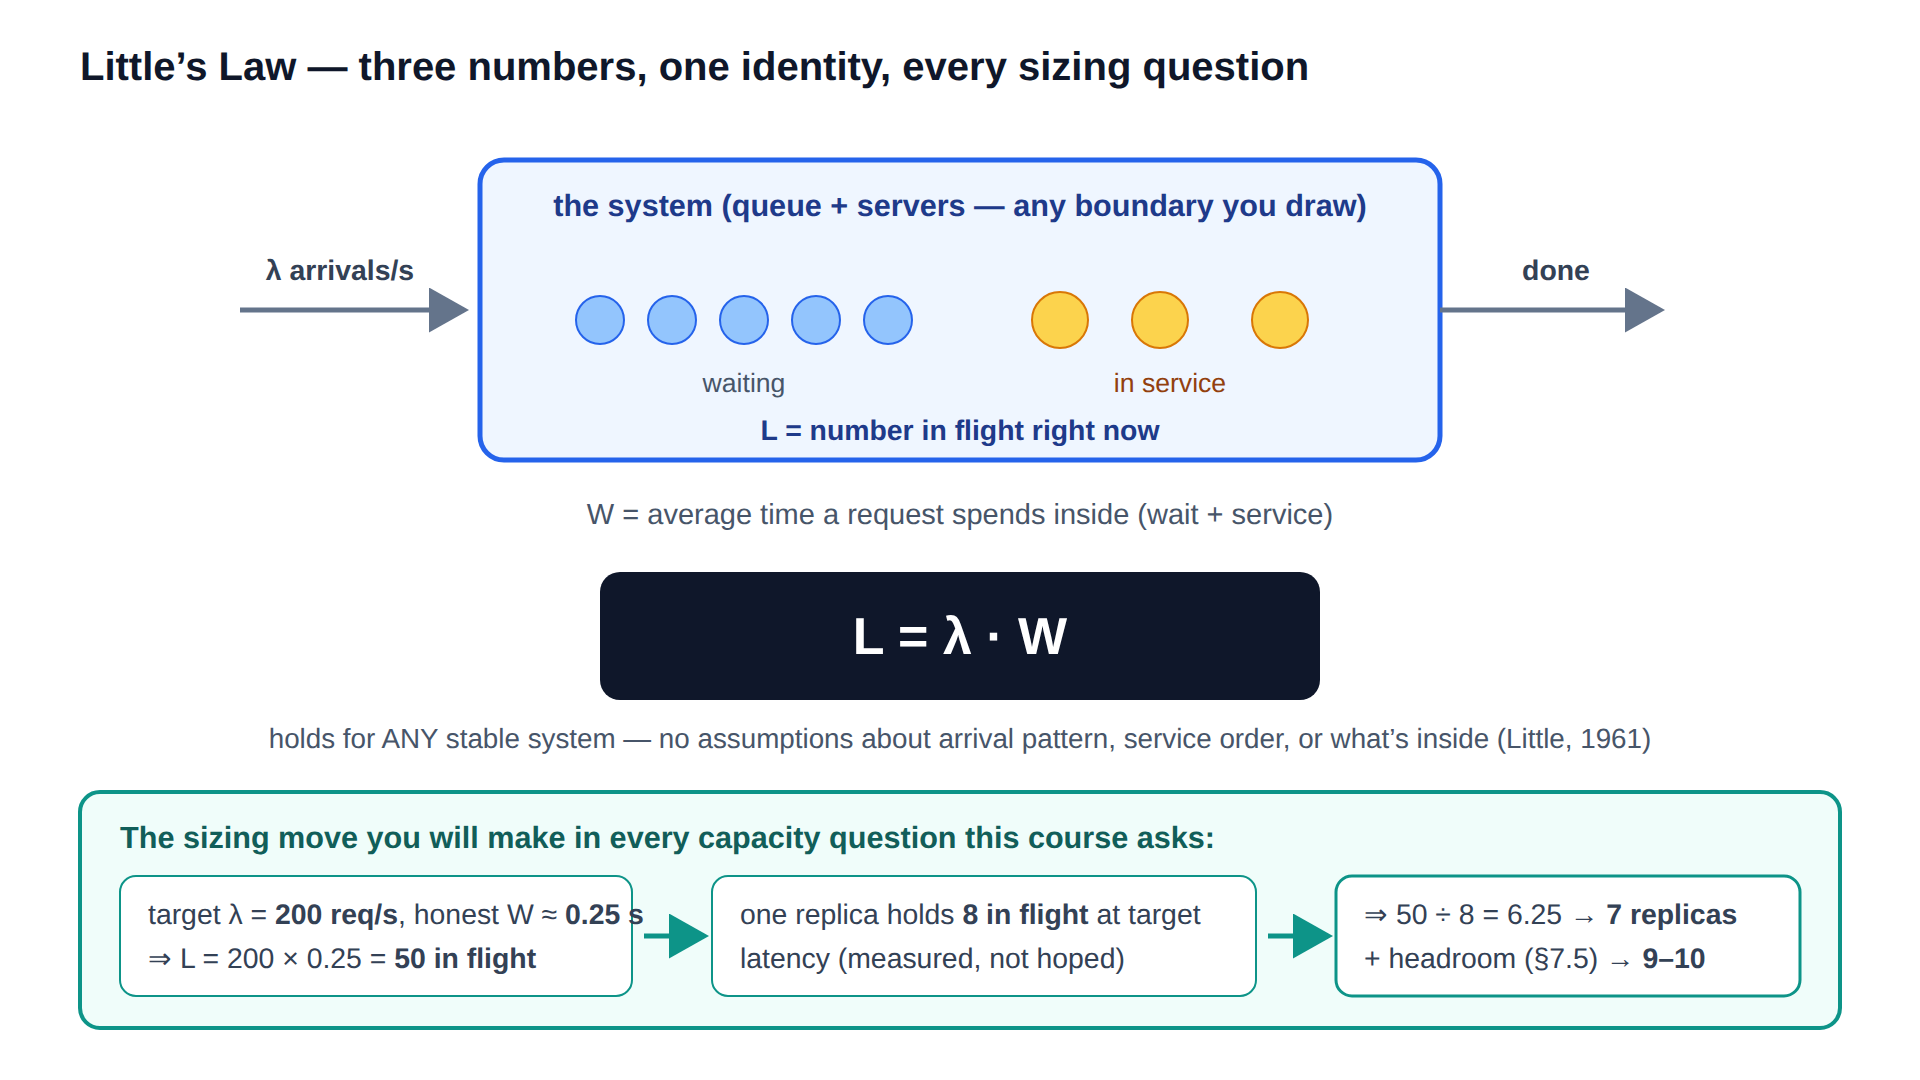
\includegraphics{figures/fig7-6_littles.png}}\\[3pt]
  \figcaption{Figure 7-6  Little's Law. Any boundary, three numbers, one identity — and, bottom, the sizing move it enables, which your proposal's capacity section performs.}
\end{tbbfigure}

Because the claim sounds too good, Transcript 7-2 checks it against a live server — one worker, a fixed 50 ms of work per request, closed-loop load at three different concurrencies:

\begin{terminalbox}
\begin{Verbatim}[breaklines=true,breakanywhere=true,fontsize=\small,formatcom=\color{tbbtermfg},codes=\tbbcodeactive]
# server: 1 worker, exactly 50 ms per request. three runs of hey:
$ hey -z 30s -c 1  http://svc/predict | grep -E "Requests/sec|Average"
  Requests/sec:  20.0      Average: 0.0500 s    # L = 20.0 x 0.050 =  1.0
$ hey -z 30s -c 10 http://svc/predict | grep -E "Requests/sec|Average"
  Requests/sec:  20.0      Average: 0.4999 s    # L = 20.0 x 0.500 = 10.0
$ hey -z 30s -c 40 http://svc/predict | grep -E "Requests/sec|Average"
  Requests/sec:  20.0      Average: 1.9998 s    # L = 20.0 x 2.000 = 40.0
# throughput is PINNED at 1/0.050 = 20/s no matter the concurrency;
# raising c only chose how much waiting existed. L = λW, every time.
\end{Verbatim}
\end{terminalbox}
\figcaption{Transcript 7-2  Little's Law, verified live. One server, one fact (50 ms per request), three concurrencies — the identity holds to the third decimal, and the throughput ceiling (1 ÷ service time) is exactly Chapter 1's Exhibit A arithmetic wearing its real name.}

Three practical uses follow immediately. \textbf{Sizing} (the big one, below): given target λ and an honest W, L = λW tells you how many requests will be in flight, and dividing by what one replica can hold in flight gives the fleet. \textbf{Sanity-checking dashboards}: your metrics claim 300 req/s at 400 ms average — then \textasciitilde{}120 requests should be in flight; if the in-flight gauge says 15, one of your three numbers is lying (usually the latency, measured in the wrong place — §7.3). \textbf{Finding hidden queues}: when measured W at the client exceeds server-side W, Little's Law applied to the gap \textit{localizes the invisible queue} — in the LB, in the kernel accept queue, in the GPU batcher — before you go hunting (the Chapter 3 debugging instinct, now quantitative).

\subsection*{The hockey stick: why systems die at 90\%}

Little's Law counts what \textit{is}; the second result predicts what \textit{happens} as you push your luck. Model one replica as a queue with random (Poisson) arrivals and exponentially distributed service — the textbook \textbf{M/M/1} queue — and define utilization \textbf{ρ = λ ÷ capacity}. The mean time in system is \textbf{W = S ÷ (1 − ρ)}, where S is the bare service time. Read the denominator: at ρ = 0.5, W = 2S — waiting already equals working. At ρ = 0.8, 5S. At 0.9, 10S. At 0.95, 20S (Figure 7-5). The curve is a hockey stick with its blade pointed at your SLO, and the physical cause is not exhaustion but \textbf{variability}: random arrivals \textit{cluster}, and near capacity there is no slack to absorb a cluster, so queues form even though average demand is below average supply. (Real serving systems are messier than M/M/1 — GPU batching, multiple workers, non-exponential service — but the shape survives every complication; only the numbers shift.)

\begin{tbbfigure}
  \adjustbox{max width=0.94\linewidth,max totalheight=0.46\textheight}{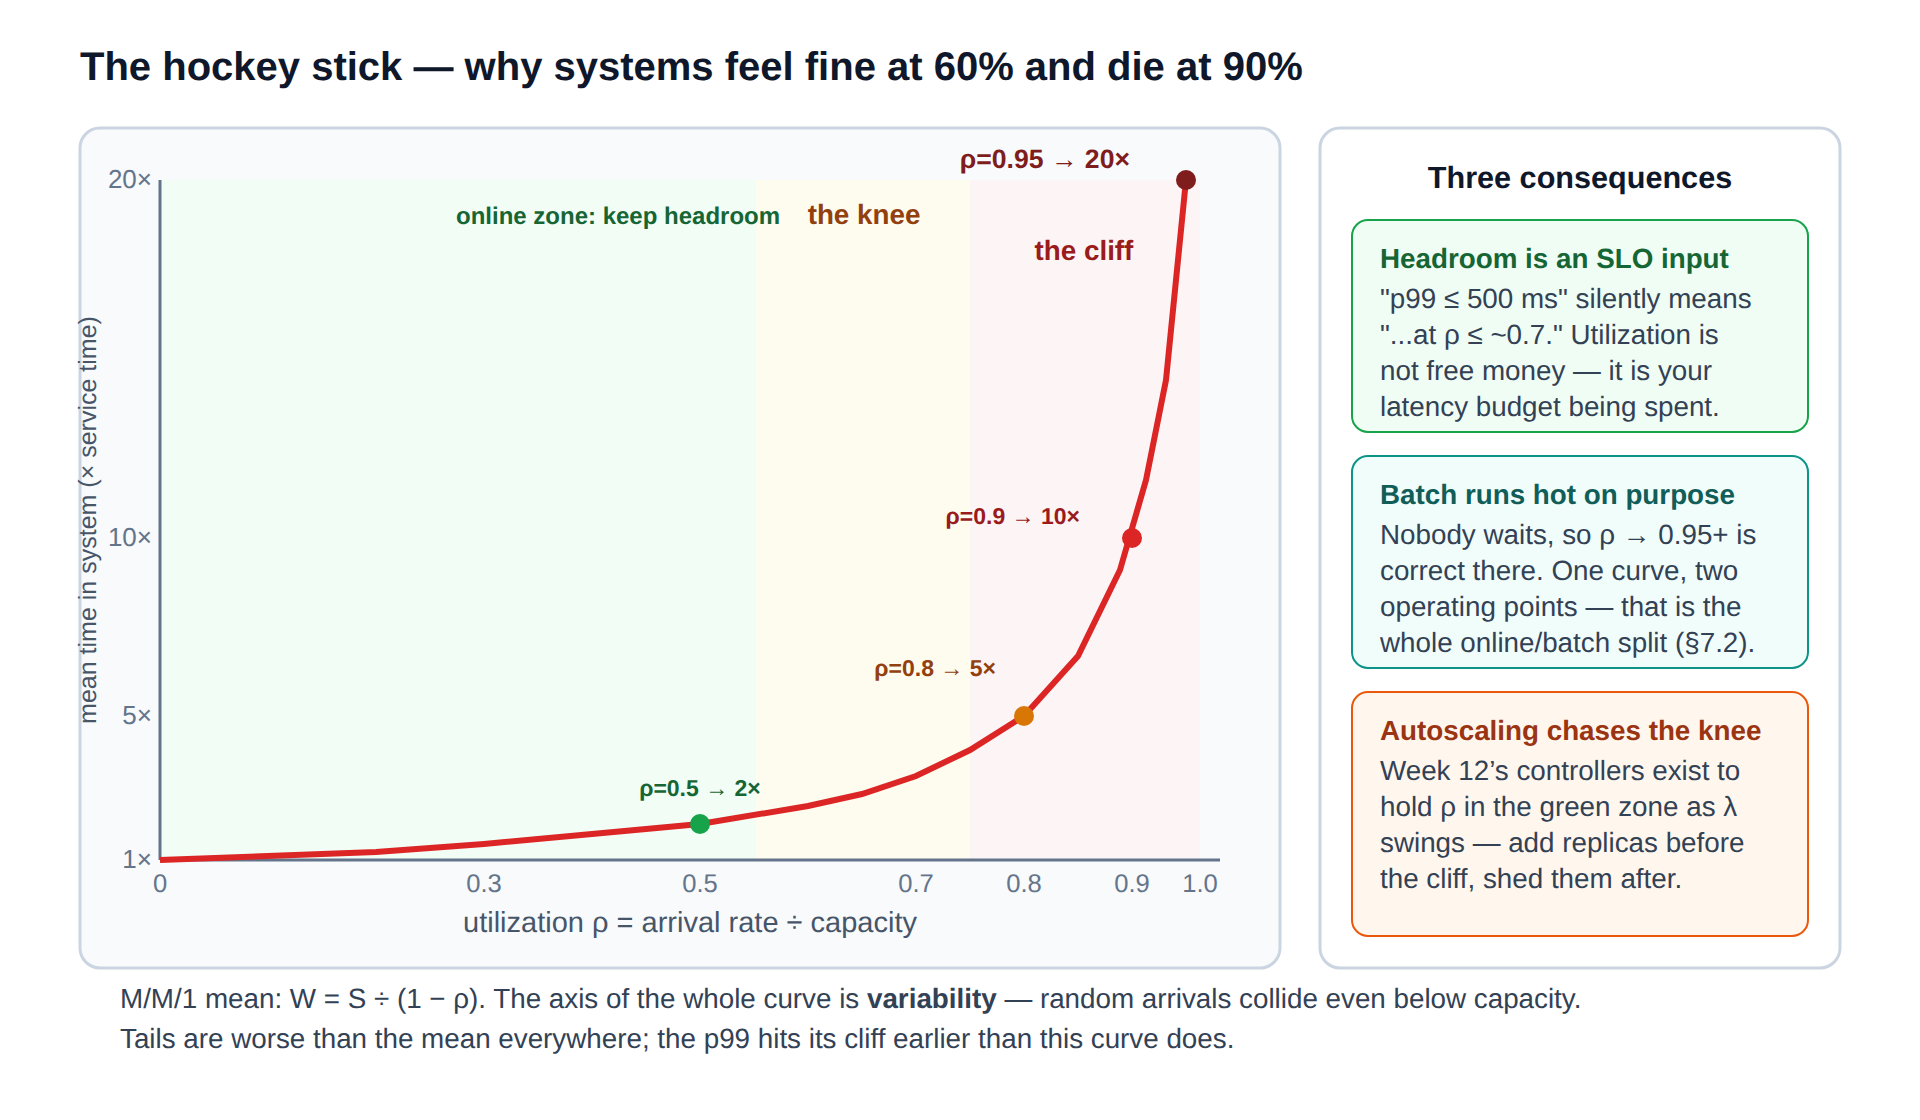
\includegraphics{figures/fig7-5_hockey.png}}\\[3pt]
  \figcaption{Figure 7-5  The hockey stick, W = S ÷ (1 − ρ), with the three operating lessons: headroom is an SLO input, batch runs hot on purpose, and autoscaling exists to chase the knee.}
\end{tbbfigure}

\begin{terminalbox}
\begin{Verbatim}[breaklines=true,breakanywhere=true,fontsize=\small,formatcom=\color{tbbtermfg},codes=\tbbcodeactive]
# same 20/s-capacity server. open-loop sweeps (wrk2), 3 min per point:
  rate      rho     p50       p99
  10.0/s    0.50     69 ms    460 ms
  16.0/s    0.80    173 ms    1.2 s
  18.0/s    0.90    347 ms    2.3 s
  19.0/s    0.95    693 ms    4.6 s     # +5% load -> +100% latency
  19.8/s    0.99    3.5 s      23 s     # queue now barely drains at all
# nothing "broke," no error was logged. arithmetic happened.
# and note the tail: p99 hits YOUR SLO long before p50 looks sick.
\end{Verbatim}
\end{terminalbox}
\figcaption{Transcript 7-3  The hockey stick, measured. Every row matches M/M/1's prediction (p50 ≈ 0.69·W, p99 ≈ 4.6·W); the operational reading is the last comment — the tail breaches the SLO while the median still looks healthy.}

Three consequences to keep (Figure 7-5, right). \textbf{Headroom is an SLO input}: a promise like "p99 ≤ 500 ms" silently carries "...at ρ ≤ \textasciitilde{}0.7," so utilization is not free money — it is your latency budget being spent; fleets that chase 95\% utilization on the online path are simply pre-spending their p99. \textbf{Batch runs hot on purpose}: with nobody waiting, ρ → 0.95 is \textit{correct} — one curve, two operating points, and that split is the entire economic argument of §7.2. \textbf{Autoscaling chases the knee}: Week 12's controllers exist to hold ρ in the green zone as λ swings, adding replicas before the cliff and shedding them after; the hockey stick is the \textit{reason} the HPA has a target-utilization field.

\subsection*{Fleet sizing, honestly — and the bill that teaches the syllabus}

Now assemble the proposal's capacity section from parts you already own. \textbf{Step 1 — measure one replica, honestly}: open-loop load (§7.3), through the gateway, sweeping rate until the SLO's latency target breaks. Suppose your quantized 3B model on one L4 replica sustains \textbf{28 req/s at p99 = 460 ms} (comfortably inside the 500 ms promise; pushing to 34 req/s blew the tail — the hockey stick in action, since 28/40-ish saturation ≈ ρ 0.7). \textbf{Step 2 — Little's cross-check}: at 200 req/s target with honest mean W ≈ 0.16 s, L = 200 × 0.16 = \textbf{32 requests in flight} fleet-wide — about 4 per replica across 8, consistent with the batcher depth you measured; if your framework's in-flight gauge disagrees wildly in Week 9's lab, something is queueing where you are not looking. \textbf{Step 3 — divide and round up}: 200 ÷ 28 = 7.1 → \textbf{8 replicas} at peak (headroom already inside the 28, because you measured \textit{at} the SLO, not at saturation).

\textbf{Step 4 — price it}, with Chapter 2's fleet table: 8 × L4 at \textasciitilde{}\$0.80/hr × 744 h = \textbf{\$4,762/month}. Your proposal's ceiling is \$900. Sit with that number for a moment, because discovering it \textit{now, on paper, for free} is this chapter's single most valuable deliverable — Exhibit 1-B's team discovered their version at month-end, in production, in dollars. And the gap is not a verdict; it is a \textbf{syllabus}: quantization (Week 10) that doubles per-replica throughput halves the fleet (→ \textasciitilde{}\$2,381); autoscaling (Week 12) that follows your diurnal curve — if the 200 req/s peak holds only \textasciitilde{}4 hours a day — roughly halves replica-hours again (→ \textasciitilde{}\$1,200); smarter batching (Weeks 10–11) and spot capacity for any batch component (Week 12) close the rest. \textbf{The road from \$4,762 to \$900 is, almost line for line, the second half of this course.} Write both numbers in the proposal: the honest today-price, and the target with the levers you intend to pull.

\begin{calloutbox}{tbbpurple}{tbbpurplefill}
{\normalsize\bfseries\color{tbbpurple}Think About It}\par\vspace{3pt}
\begin{tbbitemize}
  \item Recompute Exhibit 1-A with this section's tools: service time 0.31 s, one replica, 100 concurrent users. What are λ\_max, ρ, and W from Little's Law? Now add the gateway's 30 s timeout: what fraction of arrivals 504? (You did this by feel in Chapter 1 — now show it as a two-line calculation.)
  \item Your dashboard shows λ = 120 req/s, mean latency 250 ms, and an "in-flight requests" gauge reading 90. Use Little's Law to prove one of these three numbers is wrong, and rank the suspects (§7.3 has opinions).
  \item A teammate proposes running the online fleet at ρ = 0.9 "because idle GPUs are waste" (Chapter 1!). Using Transcript 7-3's rows, write the two-sentence rebuttal that names what ρ = 0.9 costs, and the §7.2 alternative for the workloads where their instinct is actually right.
  \item Re-derive step 4's autoscaling estimate: peak 200 req/s for 4 h/day, \textasciitilde{}60 req/s otherwise. With 28 req/s per replica, how many replica-hours per day does a perfect autoscaler use vs. the fixed fleet of 8? What does Week 12's cold-start problem do to "perfect"?
\end{tbbitemize}
\end{calloutbox}

\section{Model Formats and Conversion Paths}

One blank remains in the proposal: \textbf{what file, exactly, does the runtime execute?} Chapter 6 built the shelf — a versioned, digest-addressed prefix in the object store, fetched at startup over parallel ranged GETs — and promised that \textit{what sits on the shelf} was this week's business. The question splits cleanly in two: how the \textbf{weights} sit in a file (a solved problem with one security lesson attached), and how the \textbf{computation} ships (a live trade-off you will revisit in Week 10). Figure 7-7 is the map.

\begin{tbbfigure}
  \adjustbox{max width=0.94\linewidth,max totalheight=0.46\textheight}{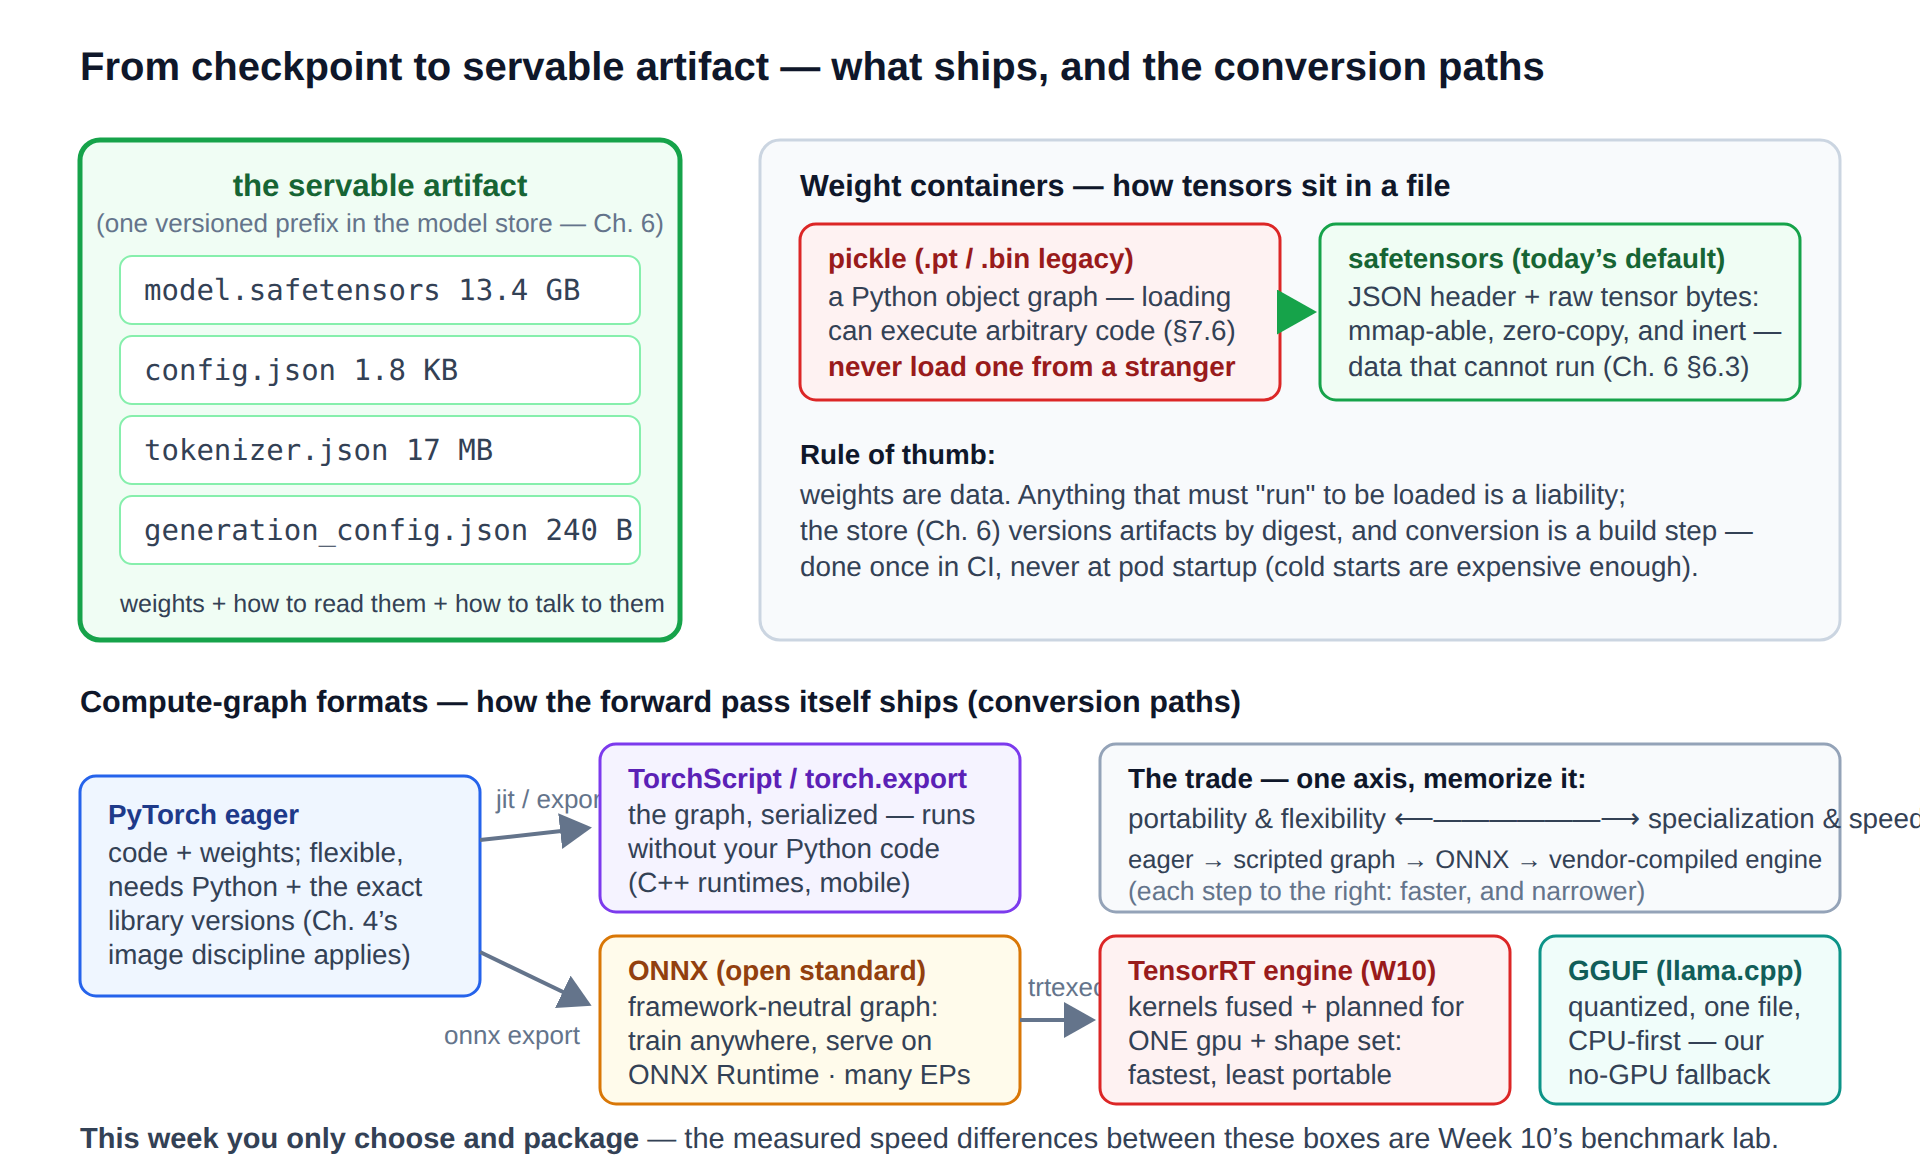
\includegraphics{figures/fig7-7_formats.png}}\\[3pt]
  \figcaption{Figure 7-7  The servable artifact and its formats. Left: what actually ships. Top: weight containers — pickle's hazard vs. safetensors. Bottom: compute-graph formats along one axis — rightward is faster and narrower.}
\end{tbbfigure}

\subsection*{The artifact: weights, plus how to read them, plus how to talk to them}

Strip any modern model directory and three roles remain (Figure 7-7, left): the \textbf{weights} (\code{model.safetensors} — the gigabytes); the \textbf{architecture config} (\code{config.json} — the kilobyte that says \textit{how to arrange} the gigabytes: layer counts, dimensions, activation choices); and the \textbf{tokenizer} (\code{tokenizer.json} — the contract between human text and tensor indices). Losing any one strands the others: weights without config are an unlabeled binary; config and weights without the \textit{exact} tokenizer produce fluent nonsense (a classic, maddening failure — the model "works" and answers in word salad, because token 4821 no longer means what training said it meant). This trio is the \textbf{servable artifact}, it versions as a unit under one digest-pinned prefix (Chapter 4's tag-vs-digest discipline, replayed on the model store), and your proposal names it explicitly: model, size, quantization state, license, artifact layout.

\subsection*{The pickle problem: a warning made real}

Chapter 6 stated it as a specification bullet — safetensors is "data that cannot run" — and promised this week would repeat it \textit{with feeling}. Here is the feeling. PyTorch's classic checkpoint format (\code{.pt}/\code{.bin}) is a \textbf{pickle}: a serialized Python \textit{object graph}, whose deserializer will happily reconstruct objects by calling functions the file names. That is not a bug in pickle — it is pickle's contract — and it means \textbf{loading a checkpoint can execute code chosen by whoever made the file}:

\begin{terminalbox}
\begin{Verbatim}[breaklines=true,breakanywhere=true,fontsize=\small,formatcom=\color{tbbtermfg},codes=\tbbcodeactive]
$ python - <<'EOF'
import pickle
class Innocent:                    # what a "checkpoint" can smuggle
    def __reduce__(self):          # pickle: "to rebuild me, call this"
        return (print, ("hello from INSIDE your checkpoint load",))
blob = pickle.dumps(Innocent())
pickle.loads(blob)                 # merely LOADING the file...
EOF
hello from INSIDE your checkpoint load
# loads() called a function the file chose. print() today;
# os.system() in a malicious "fine-tune" you downloaded tomorrow.
$ python -c "from safetensors.torch import load_file as l; l('m.safetensors')"
# JSON header parsed, tensors mmap'd. nothing executes, ever. (Ch. 6)
\end{Verbatim}
\end{terminalbox}
\figcaption{Transcript 7-4  The pickle problem, demonstrated benignly. Deserializing a pickle can call arbitrary functions named by the file — which is why "I downloaded a checkpoint" is a code-execution event, and why the ecosystem moved to safetensors.}

The operational rules that follow are short. Prefer \textbf{safetensors} everywhere (it is also \textit{faster} — the mmap/zero-copy loading of Chapter 6, no deserialization tax). Where legacy pickles are unavoidable, load with \code{torch.load(..., weights\_only=True)} — modern PyTorch defaults to it precisely because of this transcript — and treat any exception as a red flag, not an inconvenience to work around. And institutionally: model files are \textit{inputs from the internet}; give them the same trust you give a random Docker image (Chapter 4) — which is to say, provenance and digests, or nothing. (Chapter 6's security exercise — "an attacker achieves code execution inside a serving pod via a malicious pickle" — assumed this section; you can now write its first line yourself.)

\subsection*{Graph formats: one axis, four stops, and a rule about when to convert}

Weights are inert data; something must still \textit{compute}. The options line up on a single axis (Figure 7-7, bottom): each step rightward trades portability and flexibility for speed and specificity. \textbf{Eager PyTorch} ships your Python code next to the weights — maximally flexible, and maximally entangled with the environment (the exact library versions: Chapter 4's "works on my machine" disease, kept at bay only by the image discipline you already have). \textbf{TorchScript / `torch.export`} serializes the graph itself, so a C++ runtime can execute it without your Python. \textbf{ONNX} is the framework-neutral interchange: \code{torch.onnx.export} emits a standard graph that \textbf{ONNX Runtime} executes through pluggable \textit{execution providers} (CPU, CUDA, TensorRT, and friends) — train anywhere, serve anywhere, at the cost of operator-coverage edges (custom ops and exotic dynamic shapes travel poorly). \textbf{Compiled engines} — TensorRT most prominently — take a graph and \textit{plan} it for one GPU model and one shape envelope: kernels fused, precisions chosen, memory pre-arranged; fastest, and so narrow that an engine built for an A10G will not run elsewhere. (Parallel to all of this sits \textbf{GGUF}, llama.cpp's quantized single-file format — pragmatically important as this course's no-GPU fallback path.) The measured speed differences along the axis are Week 10's benchmark lab; this week you only \textit{choose and package}.

Two rules make the choice operational. \textbf{Conversion is a build step, never a startup step}: export and validation run once, in CI, producing a new digest-pinned artifact — because pod startup is already the cold-start critical path (Chapter 6 priced it), and because a conversion that happens N times per scale-out event is N chances to produce N subtly different models. And \textbf{converted models must prove equivalence}: run a fixed input battery through source and converted model and compare outputs within tolerance \textit{before} the artifact earns a version — graph conversions legitimately reorder floating-point math, so bit-equality is the wrong test, but "close within 1e-3 and identical top-1" is a five-line script that has caught real, silent numerical breakage. A conversion without an equivalence check is a model you have never actually tested.

\begin{calloutbox}{tbbpurple}{tbbpurplefill}
{\normalsize\bfseries\color{tbbpurple}Think About It}\par\vspace{3pt}
\begin{tbbitemize}
  \item Your teammate's proposal says "we will convert to TensorRT at pod startup for maximum flexibility." Give the three-part critique this section arms you with (cold start, artifact identity, equivalence testing), and the CI-shaped alternative.
  \item Why does the tokenizer belong INSIDE the versioned artifact rather than baked into the serving image? Construct the failure that occurs when model v7 ships with v6's tokenizer — what does the service return, and which of §7.4's SLIs (if any!) would even notice?
  \item Rank for your own project: eager / TorchScript / ONNX / TensorRT / GGUF. Which do you ship in the proposal, and which is your Week 10 experiment? Name the binding constraint (team skills, hardware, model architecture) that made the choice.
\end{tbbitemize}
\end{calloutbox}

\section{Lab: The Project Proposal — One Page, Five Numbers}

This week's deliverable is the team project proposal: \textbf{one page} that would have saved Exhibit 7-A's team their Wednesday meeting. Every section of this chapter filled one of its blanks; the lab is assembling them — plus one honest measurement to anchor the capacity math. The grading rubric is the sentence from Box 7-2, expanded.

\subsection*{The proposal's five sections}

\begin{tbbitemize}
  \item \textbf{1 · The artifact (§7.6).} Model, parameter count, quantization state, license, and the exact artifact layout (weights format, tokenizer, config) with its storage prefix. If your model arrives as a pickle, say how it becomes a safetensors artifact — in CI, with an equivalence check.
  \item \textbf{2 · The mode and traffic decomposition (§7.2).} Which requests are truly online, what runs batch, whether responses stream — with Table 7-2's five questions answered for your main path.
  \item \textbf{3 · The SLO sentence (§7.4).} All five clauses: SLI, target, window, load clause, cost ceiling. This sentence is the contract your Week 15 demo is graded against; the Week 12 checkpoint re-reads it.
  \item \textbf{4 · The capacity and cost envelope (§7.5).} Measured single-replica sustainable rate at the SLO (open-loop, through the gateway — Box 7-1); Little's-Law cross-check; replica count at peak; honest monthly price from Chapter 2's fleet table; and the today-price → target-price gap with the Weeks-10–12 levers you plan to pull.
  \item \textbf{5 · Risks and fallbacks.} The two classics every team should name: GPU quota/availability (fallback: smaller model, or GGUF on CPU — the course's guaranteed path), and the SLO proving unaffordable (fallback: the §7.4 loosening you would defend, chosen now, calmly, instead of at 2 a.m. in Week 14).
\end{tbbitemize}

\subsection*{The measurement that anchors it}

One number in the proposal must be \textit{measured}, not estimated: a first single-replica benchmark of \textbf{any} servable stand-in for your model (your actual candidate if it already runs; the Week 4 FastAPI lab server if not). The protocol is Box 7-1 in miniature: deploy behind the gateway; warm up and discard; open-loop sweep at 3–5 rates; record p50/p95/p99 \textit{with} the error rate at each; find the highest rate at which your draft SLO's latency target survives. That rate — requests per second per replica, at the SLO — is the seed of every capacity number you will compute for the rest of the course, and Week 9's framework lab re-measures it properly with Locust so you can watch your own tooling improve the number's honesty.

\begin{calloutbox}{tbbred}{tbbxFEF2F2}
{\normalsize\bfseries\color{tbbx991B1B}Box 7-3  The six proposal mistakes graders see every year}\par\vspace{3pt}
\begin{tbbitemize}
  \item \textbf{"Average latency ≤ X"} — an SLI this chapter spent a section dismantling. Percentiles or nothing (§7.3).
  \item \textbf{No load clause} — a p99 promised at unspecified λ promises nothing; the hockey stick eats it at the first burst (§7.5).
  \item \textbf{Accuracy as an SLO} — model quality drifts with the world, not with your infrastructure; promise validity/completion SLIs instead and monitor drift in Week 14 (§7.4, Table 7-3).
  \item \textbf{Cost = GPU only} — the meter also runs on the LB, NAT egress (Chapter 6's tax), storage, and the staging environment you forgot to terminate (Exhibit 1-B lives on).
  \item \textbf{Closed-loop benchmark numbers} — capacity measured with politely-waiting clients overstates what open-loop reality delivers; label your loop or lose the marks (§7.3, Transcript 7-1).
  \item \textbf{Conversion at startup} — the cold-start path is sacred; conversions happen in CI, once, with an equivalence check (§7.6).
\end{tbbitemize}
\end{calloutbox}

\vspace{3.0pt}

Deliverable checklist: the one-pager (five sections, five clauses in the SLO sentence), the benchmark table (rates × p50/p95/p99/error\%), and — in memory of Exhibit 1-B — a screenshot of this week's billing console showing what the measurement cost. Typical answer: under two dollars. The habit is the point.

\begin{calloutbox}{tbbpurple}{tbbpurplefill}
{\normalsize\bfseries\color{tbbpurple}Think About It}\par\vspace{3pt}
\begin{tbbitemize}
  \item Trade proposals with another team and grade only their SLO sentence against Box 7-2's checklist: which clause is missing or unmeasurable? (Every year, the most common finding is the load clause.)
  \item Your measured single-replica rate is 9 req/s at the SLO, and your target is 200 req/s: 23 replicas, \textasciitilde{}\$13,700/month on L4s. Which THREE levers from this chapter and the syllabus do you pull first, and what does each plausibly buy? (There is a right first answer, and it is not "more GPUs.")
  \item Write the 2 a.m. version: it is Week 14, your SLO is breached, the demo is in six days. Which clause of your own proposal do you invoke — and what did this chapter make you write down, back in Week 7, that makes the 2 a.m. decision a reading exercise instead of an argument?
\end{tbbitemize}
\end{calloutbox}

\namedsection{Summary}{The Chapter in Twelve Points}

\qitem{1}{\textbf{A service without an agreed number has no difference between fine and broken.} Exhibit 7-A's argument had no wrong participants — only a missing sentence. The fix is the SLI → SLO → SLA ladder, and writing that sentence is this week's deliverable.}

\qitem{2}{\textbf{Latency is a distribution, and the mean describes nobody.} Exhibit 7-B's mean (182 ms) sat between p50 (92 ms) and p90, experienced by no one, while 100 users a day lived past p99 = 2.1 s. Serving speaks percentiles: p50 is typical, p99 is a daily crowd, p99.9 is the CEO's live demo.}

\qitem{3}{\textbf{Speed is revenue} — the classics (Amazon's +100 ms → −1\% sales; Google's +400 ms → −0.59\% searches, persisting after removal; Mayer's +500 ms → −20\% traffic) replicate in direction two decades on. Latency is a line item.}

\qitem{4}{\textbf{The mode question — "who is waiting, and for what?" — shapes the whole system.} Online manages tails, batch manages cost (run hot, use spot, nobody waits), streaming manages felt speed (time-to-first + cadence). The cheapest latency optimization is discovering nobody was waiting.}

\qitem{5}{\textbf{Percentile grammar:} percentiles need a window, a place (measure where the user is), and a load; they do not add across pipeline stages; and they cannot be averaged across replicas — aggregate histograms, not percentiles (why Prometheus ships buckets, Week 14).}

\qitem{6}{\textbf{Tails multiply under fan-out} (Dean \& Barroso): 1\% slow per call × 100-way fan-out = 63\% of user requests touch a slow call. Hence shallow fan-outs, per-call timeouts, and hedged requests — cost spent to buy back the tail.}

\qitem{7}{\textbf{Load tests lie by coordinated omission:} closed-loop testers stop sending exactly when the server stalls (Transcript 7-1: p99 = 13 ms vs. the open-loop truth of 1.14 s). SLO questions require open-loop, fixed-rate load — plus Box 7-1's hygiene.}

\qitem{8}{\textbf{An SLO has five clauses} — SLI, target, window, load clause, cost ceiling — and its complement is the error budget (99.9\%/30 d ≈ 43 min): a launch/freeze policy, not a report card. 100\% is the wrong target; each nine costs \textasciitilde{}10× and vanishes into the user's noise floor.}

\qitem{9}{\textbf{Little's Law (L = λ·W) holds for any stable boundary} — the conservation law of serving. Uses: fleet sizing, dashboard sanity checks (λ·W must equal in-flight), and localizing hidden queues. It is Chapter 1's Exhibit A arithmetic, formalized.}

\qitem{10}{\textbf{The hockey stick (W = S ÷ (1−ρ)) is why systems die at 90\%:} waiting equals working already at ρ = 0.5, and doubles again from ρ = 0.9 to 0.95. Headroom is an SLO input; batch runs hot on purpose; autoscaling exists to chase the knee (Week 12).}

\qitem{11}{\textbf{Fleet sizing is measurement + division:} single-replica rate at the SLO (open-loop, at the gateway) → replicas = ceil(target λ ÷ per-replica rate) → price it with the fleet table. Our worked example's first bill (\$4,762 vs. a \$900 ceiling) is not a failure — the gap is the syllabus of Weeks 10–12.}

\qitem{12}{\textbf{The servable artifact = weights + config + tokenizer, versioned as one digest-pinned unit.} Pickle checkpoints can execute code on load (Transcript 7-4) — prefer safetensors, \code{weights\_only=True} otherwise. Graph formats trade portability for speed (eager → TorchScript → ONNX → TensorRT; GGUF as the CPU fallback); conversion is a CI build step with an equivalence check, never a pod-startup step.}

\namedsection{Exercises}{}

\subsection*{A. Multiple choice}

\qitem{1}{A pipeline re-embeds the entire document corpus every night; results must be ready by 06:00. No user ever awaits an individual embedding. Which mode and utilization stance fit?}

\begin{tbboptions}
  \item ① Online — keep ρ ≤ 0.7 for the tail        ② Batch — run GPUs hot (ρ → 0.95), spot-friendly, deadline SLO
  \item ③ Streaming — optimize time-to-first-embedding        ④ Online — because the 06:00 deadline is a latency target
\end{tbboptions}

\qitem{2}{In Exhibit 7-B (10,000 requests, p50 = 92 ms, mean = 182 ms, p99 = 2,140 ms), which statement is correct?}

\begin{tbboptions}
  \item ① About 100 of the 10,000 requests took longer than 2,140 ms
  \item ② Most users experienced roughly 182 ms
  \item ③ The p99 must be wrong, because it exceeds 10× the mean
  \item ④ Half the requests took longer than 182 ms
\end{tbboptions}

\qitem{3}{Each of 10 downstream calls in a fan-out is slow 1\% of the time, independently, and the request waits for all of them. Roughly what fraction of user requests hit at least one slow call?}

\begin{tbboptions}
  \item ① 0.1\%        ② 1\%        ③ \textasciitilde{}10\%        ④ 63\%
\end{tbboptions}

\qitem{4}{A server stalls completely for 1.5 s once a minute. Which load-testing setup will reveal the stall in its reported p99?}

\begin{tbboptions}
  \item ① Closed-loop, 64 concurrent connections, 2-minute run
  \item ② Closed-loop with more connections (256)
  \item ③ Open-loop at a fixed arrival rate near capacity, several minutes
  \item ④ Any tool, provided the run is long enough
\end{tbboptions}

\qitem{5}{Which of the following is a complete SLO by §7.4's anatomy?}

\begin{tbboptions}
  \item ① "p99 ≤ 500 ms" 
  \item ② "99.5\% of requests under 500 ms at the gateway, per rolling 30 days, at up to 200 req/s, under \$900/month"
  \item ③ "average latency ≤ 200 ms and 99.99\% availability, forever"
  \item ④ "as fast as possible at all times"
\end{tbboptions}

\qitem{6}{Your availability SLO is 99.9\% over 30 days (\textasciitilde{}43 min budget). An incident on day 9 consumed 50 minutes. Per the error-budget policy, what happens?}

\begin{tbboptions}
  \item ① Nothing; budgets are advisory
  \item ② Launches freeze and effort shifts to reliability until the rolling window recovers — by prior agreement
  \item ③ The SLO is retroactively loosened to fit the incident
  \item ④ The error budget resets immediately after any postmortem
\end{tbboptions}

\qitem{7}{A service receives λ = 80 req/s with mean time-in-system W = 0.3 s. How many requests are in flight on average (Little's Law)?}

\begin{tbboptions}
  \item ① 24        ② 267        ③ 80        ④ Cannot be determined without the arrival distribution
\end{tbboptions}

\qitem{8}{An online fleet runs at ρ = 0.9 (mean latency ≈ 10× service time, M/M/1). Traffic grows 5\% so ρ ≈ 0.95. What does the model predict for mean latency?}

\begin{tbboptions}
  \item ① +5\%, matching the load growth        ② Roughly doubles, to \textasciitilde{}20× service time
  \item ③ Unchanged until ρ = 1.0        ④ +50\%
\end{tbboptions}

\subsection*{B. Short answer}

\qitem{1}{Name the load-testing pathology in which the tool stops generating load precisely while the server stalls, and state in one sentence why the reported percentiles are wrong.}

\qitem{2}{Target load is 120 req/s; one replica sustains 25 req/s at the SLO's latency target (measured open-loop). How many replicas at peak, and why is no extra headroom factor needed on top?}

\qitem{3}{In one sentence each: why can loading a legacy .pt checkpoint execute attacker-chosen code, and why can a safetensors file not?}

\qitem{4}{Compute the 30-day error budget, in minutes, for an availability SLO of 99.5\%.}

\qitem{5}{List the five mandatory clauses of a complete SLO sentence in this course.}

\subsection*{C. Essay}

\qitem{1}{Rewrite Exhibit 7-A as an incident narrative in a team that has adopted §7.4's machinery: the PM's report, the engineer's data-bearing reply (SLI, current burn, histogram evidence per §7.3), and the decision the error-budget policy produces. Then state, in one paragraph, what organizational argument the machinery eliminated and what engineering argument it deliberately preserved.}

\qitem{2}{Design the capacity section of a proposal: measured 22 req/s per L4 replica at the SLO; peak 150 req/s for \textasciitilde{}3 h/day, \textasciitilde{}40 req/s otherwise; L4 ≈ \$0.8/hr. Compute the fixed-fleet monthly cost and an idealized autoscaled cost; recommend one (or a hybrid), naming the risk autoscaling introduces (Week 12 preview) and the §7.4 clause that protects you while it is unsolved.}

\qitem{3}{A document-QA product: nightly corpus embedding; per-query retrieval + reranking inside the request; answers streamed token-by-token. Decompose it by §7.2's modes, choose an SLI and target for each component (Table 7-3), and identify which component's tail dominates the user's experience under §7.3's fan-out logic.}

\qitem{4}{Defend a formats plan for your project: source checkpoint format and its risks (§7.6), the serving format you ship Week 9, the conversion you will attempt in Week 10, where each conversion runs (CI vs. startup — justify), and the equivalence test that gates promotion. Include the GGUF/CPU fallback and state what SLO change it would force.}

\namedsection{Answers and Commentary}{}

\subsection*{A. Multiple choice}

\qitem{1}{\textbf{②} Nobody awaits an item, so it is batch: run hot, tolerate interruption (spot), and promise the deadline as a freshness SLO ("output complete by 06:00, ≥ 99\% of mornings"). ④ confuses a job deadline with per-request latency. (§7.2)}

\qitem{2}{\textbf{①} p99 = 2,140 ms means 1\% of 10,000 — about 100 requests — were slower. ② is the mean fallacy (the mean sat between p50 and p90, describing nobody); ④ confuses mean with median; ③ is wishful thinking — heavy tails routinely put p99 at 10–20× the mean. (§7.3)}

\qitem{3}{\textbf{③} 1 − 0.99¹⁰ ≈ 9.6\%. The 63\% figure (④) is the 100-way fan-out from the text — a tenth of the fan-out is still a tenfold amplification of the per-call 1\%. Tails multiply. (§7.3)}

\qitem{4}{\textbf{③} Only open-loop load keeps arriving during the stall, so the queue that real users would form is measured (Transcript 7-1). More closed-loop connections (②) samples the stall slightly more but still pauses with the server; run length (④) does not fix the omission — the tool omits \textit{during} every stall regardless. (§7.3)}

\qitem{5}{\textbf{②} It has all five clauses: SLI (fraction under 500 ms at the gateway), target (99.5\%), window (rolling 30 d), load clause (≤ 200 req/s), cost ceiling (\$900/mo). ① lacks window/load/cost; ③ uses a mean, an unaffordable nine-count, and no window that ends; ④ is Exhibit 7-A. (§7.4)}

\qitem{6}{\textbf{②} The budget (≈ 43 min) is spent and then some, so the pre-agreed policy fires: freeze launches, do reliability work until the rolling window recovers. That the consequence was agreed \textit{before} the incident is the entire political value of the mechanism. (§7.4)}

\qitem{7}{\textbf{①} L = λ·W = 80 × 0.3 = 24. And ④ is the trap the law's generality removes: Little's Law needs no distributional assumptions at all — that is why it is safe to use on dashboards. (§7.5)}

\qitem{8}{\textbf{②} W = S ÷ (1−ρ): at 0.9, 10S; at 0.95, 20S — a 5\% load increase doubles latency near the cliff. This asymmetry is why headroom is an SLO input and why autoscalers act on utilization, not on latency alone (by the time latency moves, you are on the cliff). (§7.5)}

\subsection*{B. Short answer}

\qitem{1}{\textbf{Coordinated omission.} The tool's in-flight requests stall with the server, so almost no samples are recorded during exactly the periods users would have queued — percentiles are computed over a survivor population that excludes the worst experiences. (§7.3)}

\qitem{2}{ceil(120 ÷ 25) = \textbf{5 replicas.} The 25 req/s was measured \textit{at} the SLO's latency target, not at saturation — the headroom (the distance to the hockey stick's cliff) is already inside the number. Adding another factor would double-count it. (§7.5)}

\qitem{3}{A .pt is a pickle: deserialization reconstructs a Python object graph by calling functions the file names (\code{\_\_reduce\_\_}), so loading runs code the file's author chose. safetensors is a JSON header plus raw tensor bytes — pure data, mmap'd into place; there is no execution step to abuse. (§7.6)}

\qitem{4}{0.5\% of 30 days: 43,200 min × 0.005 = \textbf{216 minutes} (3.6 hours). One reason 99.5\% is a defensible student SLO and 99.99\% (≈ 4.3 min) is not. (§7.4)}

\qitem{5}{\textbf{SLI · target · window · load clause · cost ceiling.} ("Fraction of requests < 500 ms at the gateway" · "≥ 99.5\%" · "rolling 30 days" · "at up to 200 req/s" · "under \$900/month.") (§7.4)}

\subsection*{C. Essay (grading points)}

\qitem{1}{Look for: the engineer's reply citing the \textit{defined SLI} (not a mean), current window burn ("28 of 43 minutes spent" or a latency-SLI equivalent), and histogram evidence locating the CEO's sample (p99.9); a decision that follows mechanically from the budget (freeze or ship); and the closing distinction — the machinery eliminated the \textit{"is it slow?"} argument (now arithmetic) while preserving the \textit{"what should we promise?"} argument (a product decision, properly fought at proposal time). Bonus: noticing the PM's complaint channel is itself a biased tail sample (§7.1). (§§7.1, 7.3, 7.4)}

\qitem{2}{Fixed fleet: ceil(150/22) = 7 replicas × \$595/mo ≈ \textbf{\$4,166}. Idealized autoscale: 7 replicas × 3 h + ceil(40/22) = 2 replicas × 21 h ≈ 63 replica-hours/day vs. 168 → \textasciitilde{}37\%, ≈ \textbf{\$1,560/mo}. A strong answer recommends autoscaling-with-floor (never below 2), names the risk — cold starts: new replicas take minutes to pull images and load weights, so a burst outruns the scaler (Week 12; Chapter 6 priced the pull) — and invokes the SLO's load clause as the contractual protection while scaling is unsolved: the promise holds only to the stated λ. (§7.5)}

\qitem{3}{Decomposition: corpus embedding = batch (freshness SLO, run hot, spot-friendly); retrieval + rerank = online (tail SLI at the gateway; the fan-out members); token generation = streaming (time-to-first-token + completion-fraction SLIs). The user's felt latency is dominated by the \textit{online fan-out} ahead of the stream: retrieval + rerank are serial prerequisites to the first token, so their p99s gate TTFT (percentiles don't add, but the slowest prerequisite dominates); the stream then hides the rest. Full credit connects that observation to keeping the pre-stream fan-out shallow and tightly timed out. (§§7.2, 7.3)}

\qitem{4}{Look for: source risk named honestly (pickle → Transcript 7-4; or safetensors from a hub with digest pinning); a defensible Week 9 ship (eager or TorchScript for flexibility; GGUF if CPU-bound); a Week 10 experiment (ONNX Runtime or TensorRT) with the portability-vs-speed trade stated; conversion in CI with digest-pinned outputs and the startup path explicitly conversion-free (cold-start argument); an equivalence gate (fixed input battery, tolerance + top-1 agreement); and the GGUF fallback's SLO consequence quantified qualitatively (CPU inference → looser latency target or lower load clause — an honest §7.4 renegotiation, chosen in advance). (§7.6)}

\namedsection{Further Reading}{}

Entries tagged \textbf{[This week]} are required or strongly recommended now; a \textbf{[Wk N]} tag marks material that pays off in that later week.

\begin{tbbitemize}
  \item \textbf{[This week] Google SRE Book (2016), Chapter 4, "Service Level Objectives"} — freely readable online; the canonical source of the SLI/SLO/SLA ladder and error budgets this chapter adopted wholesale. Read it before writing your proposal's SLO sentence; Appendix "Embracing Risk" (Ch. 3) pairs well.
  \item \textbf{[This week] J. Dean \& L. A. Barroso, "The Tail at Scale," CACM 2013} — eight pages; the fan-out arithmetic, why tails resist averaging, and the hedged/tied-request mitigations. The most quoted serving-systems paper of its decade, and the origin of §7.3's 63\%.
  \item \textbf{[This week, fun] Gil Tene, "How NOT to Measure Latency" (talk, various years; HdrHistogram docs)} — the coordinated-omission lecture, delivered with showman's glee. After it you will never trust a closed-loop p99 again; wrk2 and HdrHistogram are the take-home tools.
  \item \textbf{The speed-is-revenue classics} — G. Linden's 2006 talk notes ("Make Data Useful," the +100 ms Amazon experiment), J. Brutlag, "Speed Matters for Google Web Search" (2009), and M. Mayer's Web 2.0 2006 talk (the 30-results story). Short, old, and still the citations everyone reaches for; read critically per §7.1's caveats.
  \item \textbf{J. D. C. Little, "A Proof for the Queuing Formula L = λW," Operations Research 9(3), 1961} — the original; surprisingly readable. For the broader toolkit at textbook depth, L. Kleinrock, \textit{Queueing Systems, Vol. 1} (1975) remains the standard reference — far beyond this course's needs, but the M/M/1 chapter grounds §7.5 rigorously.
  \item \textbf{[Wk 9] Locust documentation (constant-throughput load shapes)} — next week's lab tool; note how open-loop arrival is expressed, and wire Box 7-1's checklist into your locustfile from day one.
  \item \textbf{[Wk 10] ONNX \& ONNX Runtime docs (execution providers) · TensorRT developer guide (builder, engines) · safetensors format spec} — the §7.6 boxes at implementation depth; skim now, benchmark in Week 10's lab.
  \item \textbf{PyTorch security note on `torch.load` and `weights\_only`} — the official statement of Transcript 7-4's lesson, including the sanctioned migration path for legacy checkpoints.
\end{tbbitemize}

\vspace{5.0pt}

\begin{calloutbox}{tbbblue}{tbbbluefill}
{\normalsize\bfseries\color{tbbblue}Next week — the midterm; then Chapter 9: Model Serving Frameworks}\par\vspace{3pt}
\textbf{Week 8 is the midterm}, covering Weeks 1–7: the platform (virtualization, containers, Kubernetes, storage/networking) and this chapter's serving vocabulary. The best preparation is the one this book has been engineering all along: re-run the transcripts (every dark box from Transcript 2-1 to 7-4 is reproducible), and walk the souvenirs — exit 137, PID 41288, the 1956 box, the fleet table, the triangle, and now L = λW. If you can explain each souvenir's chapter \textit{and} its return appearances, you are ready.

\textbf{Chapter 9} puts a professional serving frame under your model: Triton Inference Server, TorchServe, BentoML, and Ray Serve — what a "serving framework" actually adds over your Week 4 FastAPI server (dynamic batching, model management, metrics endpoints, multi-model routing), how to choose among them, and a Locust load test that makes your proposal's capacity numbers honest. Bring this chapter's percentile discipline; it is about to meet its tooling.
\end{calloutbox}
